\PassOptionsToPackage{english}{babel}
\documentclass[12pt, a4paper, oneside]{abntex2}

% --- Pacotes ---
\usepackage[utf8]{inputenc}
\usepackage[T1]{fontenc}
\usepackage{lmodern}
\usepackage{microtype}
\usepackage{indentfirst}
\usepackage{graphicx}
\usepackage{xcolor}
\usepackage{amsmath}
\usepackage{hyperref}
\hypersetup{colorlinks=true, linkcolor=blue!60!black, citecolor=blue!60!black, urlcolor=blue!60!black}
\usepackage{caption}
\captionsetup[figure]{position=top}
\usepackage{float}
\usepackage{url}
\usepackage{tikz}
\usetikzlibrary{arrows.meta, positioning, calc, fit}
\usepackage{pifont}
\usepackage{circuitikz}
\usepackage{pgf-umlcd}
\usepackage{pgf-umlsd}
\renewcommand{\umldrawcolor}{black}
\renewcommand{\umlfillcolor}{white}
\usepackage{minted}
\usepackage[acronym, nomain, nopostdot]{glossaries}
\usepackage[alf]{abntex2cite}

% --- Estilo para trechos de código ---
\setminted{fontsize=\footnotesize, breaklines=true, frame=single, tabsize=4, linenos=true, numbersep=5pt}

% --- Floats para código: Algoritmo (biblioteca) e Exemplo (uso) ---
\floatstyle{plaintop}
\newfloat{algoritmo}{H}{loa}
\floatname{algoritmo}{Algoritmo}

\floatstyle{plaintop}
\newfloat{exemplo}{H}{loe}
\floatname{exemplo}{Exemplo}

% --- Quadros: saídas textuais do simulador ---
\floatstyle{plaintop}
\newfloat{quadro}{H}{loq}
\floatname{quadro}{Quadro}

% --- Lista de abreviaturas e siglas ---
\makeglossaries
\newacronym{hdl}{HDL}{\textit{Hardware Description Language}}
\newacronym{vhdl}{VHDL}{\textit{VHSIC Hardware Description Language}}
\newacronym{poo}{POO}{Programação Orientada a Objetos}
\newacronym{fpga}{FPGA}{\textit{Field-Programmable Gate Array}}
\newacronym{ide}{IDE}{\textit{Integrated Development Environment}}
\newacronym{asic}{ASIC}{\textit{Application-Specific Integrated Circuit}}
\newacronym{ula}{ULA}{Unidade Lógica e Aritmética}
\newacronym{ufsc}{UFSC}{Universidade Federal de Santa Catarina}

% --- Informações do documento ---
\titulo{Uma Biblioteca de Simulação de Circuitos Digitais em Python com Propagação Reativa}
\autor{Cainã Rinaldi Esteche}
\local{Florianópolis}
\data{2026}
\instituicao{Universidade Federal de Santa Catarina -- UFSC}
\orientador[Orientadora]{Profa. Dra. Cristina Meinhardt}
\coorientador[Coorientador]{Prof. Dr. Ismael Seidel}
\tipotrabalho{Trabalho de Conclusão de Curso}
\preambulo{Trabalho de Conclusão de Curso apresentado ao curso de Ciência da Computação da Universidade Federal de Santa Catarina como requisito parcial para obtenção do título de Bacharel em Ciência da Computação.}

\begin{document}

% --- Capa ---
\begin{capa}
  \centering
  
\includegraphics[width=3.2cm]{figuras/brasao_ufsc_crest.png}\par
  \vspace{0.5cm}
  {\ABNTEXchapterfont\large
  UNIVERSIDADE FEDERAL DE SANTA CATARINA\\
  CENTRO TECNOLÓGICO\\
  DEPARTAMENTO DE INFORMÁTICA E ESTATÍSTICA\\
  CURSO DE GRADUAÇÃO EM CIÊNCIA DA COMPUTAÇÃO}

  \vspace{2cm}
  {\ABNTEXchapterfont\large\imprimirautor}

  \vfill
  \begin{center}
  \ABNTEXchapterfont\bfseries\LARGE\imprimirtitulo
  \end{center}
  \vfill

  \large\imprimirlocal

  \large\imprimirdata

  \vspace*{1cm}
\end{capa}

% --- Folha de rosto ---
\imprimirfolhaderosto

% --- Resumo ---
\begin{resumo}
Estudantes de Ciência da Computação frequentemente enfrentam uma transição abrupta entre a programação em Python, aprendida na disciplina de Programação Orientada a Objetos, e a descrição de hardware em VHDL, exigida logo nos primeiros contatos com a disciplina de Circuitos e Técnicas Digitais. Essa transição é dificultada pela sintaxe formal e pelo modelo de execução concorrente das HDLs, por ambientes de desenvolvimento pesados e por tempos de compilação/síntese elevados, barreiras que se somam à dificuldade dos próprios conceitos de circuitos digitais. Este trabalho propõe um simulador de circuitos digitais implementado inteiramente em Python, sem dependências externas, baseado em um modelo de \textbf{propagação reativa de sinais} construído sobre o padrão de projeto \textit{Observer}: cada componente do circuito (sinal, porta lógica, somador, registrador) notifica automaticamente os componentes conectados a ele sempre que sua saída muda, propagando mudanças em cadeia de forma análoga à de um circuito físico. O simulador foi organizado em pacotes que separam representação de sinais, portas lógicas elementares e componentes compostos, incluindo um somador completo (\textit{full adder}) e um somador de N bits (\textit{ripple-carry adder}) construídos inteiramente a partir de portas lógicas, um somador alternativo baseado em conversão para inteiro (que demonstra a possibilidade de misturar Python ``puro'' com o restante do circuito reativo) e um registrador sensível a borda de \textit{clock}, tanto em uma versão abstrata em lógica Python (\texttt{BehavioralRegister}) quanto em uma versão construída inteiramente com \textit{latches}. A validação foi realizada comparando a saída do simulador ao comportamento teoricamente esperado para um conjunto de circuitos de exemplo (portas lógicas, meio-somador, somador completo, três contadores binários e um \textit{flip-flop} \textit{toggle}), verificada também por testes automatizados, incluindo o tratamento do \textit{overflow} de um contador de N bits em suas duas formas: truncamento explícito no somador baseado em inteiros e propagação natural via sinal de \textit{carry-out} no somador baseado em portas lógicas. Os resultados obtidos confirmam que a abordagem reproduz corretamente os conceitos introdutórios de circuitos digitais em um ambiente de execução já familiar ao estudante, evidenciando seu potencial como etapa preparatória de aprendizado antes do contato com HDLs tradicionais.

\vspace{\onelineskip}
\noindent
\textbf{Palavras-chave}: Circuitos digitais. Programação reativa. Padrão Observer. Python. Simulação. VHDL.
\end{resumo}

% --- Abstract ---
\begin{resumo}[Abstract]
 \begin{otherlanguage*}{english}
Computer Science students often face an abrupt transition between programming in Python, learned in the Object-Oriented Programming course, and describing hardware in VHDL, required early in the Digital Circuits and Techniques course. This transition is made harder by the formal syntax and concurrent execution model of HDLs, by heavyweight development environments, and by long compilation/synthesis times, barriers that add to the difficulty of the digital circuit concepts themselves. This work proposes a digital circuit simulator implemented entirely in Python, with no external dependencies, based on a \textbf{reactive signal propagation} model built on top of the Observer design pattern: each circuit component (signal, logic gate, adder, register) automatically notifies the components connected to it whenever its output changes, propagating changes in a chain analogous to a physical circuit. The simulator is organized into packages that separate signal representation, elementary logic gates, and composite components, including a full adder and an N-bit adder (ripple-carry adder) built entirely from logic gates, an alternative adder based on integer conversion (demonstrating that the simulator allows mixing ``plain'' Python with the rest of the reactive circuit), and a register sensitive to the clock's rising edge, both as an abstract version written in plain Python logic (\texttt{BehavioralRegister}) and as a version built entirely from latches. Validation was performed by comparing the simulator's output to the theoretically expected behavior for a set of example circuits (logic gates, half adder, full adder, three binary counters, and a toggle flip-flop), also checked by automated tests, including the handling of N-bit counter overflow in its two forms: explicit truncation in the integer-based adder and natural propagation via a carry-out signal in the gate-based adder. The results confirm that the approach correctly reproduces introductory digital circuit concepts in an execution environment already familiar to the student, showing its potential as a preparatory learning stage before contact with traditional HDLs.

\vspace{\onelineskip}
\noindent
\textbf{Keywords}: Digital circuits. Reactive programming. Observer pattern. Python. Simulation. VHDL.
 \end{otherlanguage*}
\end{resumo}

% --- Listas ---
\pdfbookmark[0]{\listfigurename}{lof}
\listoffigures
\cleardoublepage

\pdfbookmark[0]{\listtablename}{lot}
\listoftables
\cleardoublepage

\pdfbookmark[0]{Lista de Quadros}{loq}
\listof{quadro}{Lista de Quadros}
\cleardoublepage

\pdfbookmark[0]{Lista de Algoritmos}{loa}
\listof{algoritmo}{Lista de Algoritmos}
\cleardoublepage

\pdfbookmark[0]{Lista de Exemplos}{loe}
\listof{exemplo}{Lista de Exemplos}
\cleardoublepage

% --- Lista de abreviaturas e siglas ---
\pdfbookmark[0]{Lista de abreviaturas e siglas}{loabbr}
\printglossary[type=\acronymtype, title={Lista de Abreviaturas e Siglas}, style=long]
% O estilo "long" do glossaries usa longtable internamente, que incrementa
% o contador de "table" sem gerar entrada na Lista de Tabelas -- sem esta
% correcao, a primeira tabela real do documento seria numerada "2".
\addtocounter{table}{-1}
\cleardoublepage

% --- Sumário ---
\tableofcontents
\cleardoublepage

% ====================================================================
\textual
% ====================================================================

\chapter{Introdução}
\label{cap:introducao}

Circuitos digitais formam a base de praticamente todos os sistemas computacionais modernos, e seu estudo é parte obrigatória da formação em Ciência da Computação. No currículo do curso de Ciência da Computação da \gls{ufsc}, esse conteúdo é introduzido na disciplina de Circuitos e Técnicas Digitais, na qual os estudantes têm o primeiro contato formal com portas lógicas, álgebra booleana, circuitos combinacionais e sequenciais, e com uma \gls{hdl}, tipicamente \gls{vhdl}.

Paralelamente, é comum que esses mesmos estudantes estejam cursando, no mesmo período ou em período próximo, a disciplina de \gls{poo}, que utiliza Python como linguagem principal. O resultado é que o aluno transita, dentro de um curto intervalo de tempo, entre dois paradigmas de programação extremamente distintos: de um lado, Python, uma linguagem imperativa, sequencial, de sintaxe enxuta e com um ciclo de desenvolvimento quase instantâneo (editar, executar, ver o resultado); de outro, VHDL, uma linguagem declarativa e concorrente, com sintaxe verbosa e formal, que descreve \textit{hardware} e não um programa a ser executado passo a passo.

A motivação deste trabalho nasce justamente dessa distância entre as duas experiências de aprendizado vividas pelo estudante de Ciência da Computação. Observam-se, na prática, algumas dificuldades recorrentes:

\begin{itemize}
    \item \textbf{Distância de paradigma e de sintaxe}: enquanto em Python o aluno já está habituado a um código curto e direto, VHDL exige a declaração explícita de entidades, arquiteturas, sinais, tipos e processos antes mesmo de descrever a lógica desejada. Essa sintaxe extensa e formal, combinada com um modelo de execução concorrente pouco intuitivo para quem só programou de forma sequencial, torna os primeiros contatos com a disciplina de Circuitos e Técnicas Digitais particularmente custosos;
    \item \textbf{Ambientes de desenvolvimento pesados e pouco ágeis}: as \glspl{ide} tradicionalmente utilizadas para VHDL (como Quartus, da Intel, ou Vivado, da Xilinx/AMD) são ferramentas robustas, voltadas para síntese em \glspl{fpga} reais, porém pesadas, lentas para abrir e configurar, e com uma curva de aprendizado própria que é somada à da linguagem em si;
    \item \textbf{Tempo de compilação/síntese elevado}: diferentemente do ciclo quase instantâneo de ``salvar e rodar'' ao qual o aluno está acostumado em Python, a simulação ou síntese de um circuito VHDL pode levar segundos a minutos, mesmo para exemplos simples. Esse tempo de espera atrapalha a experimentação rápida e a construção de intuição sobre o comportamento do circuito, que é justamente o tipo de aprendizado que se beneficia de iteração rápida e \textit{feedback} imediato;
    \item \textbf{O problema não é exclusivo do VHDL}: linguagens de descrição de \textit{hardware} aparentadas, como Verilog e SystemVerilog, compartilham a mesma natureza concorrente, sintaxe formal e ecossistema de ferramentas pesado, de modo que a dificuldade relatada aqui não é uma particularidade do VHDL, mas sim das HDLs tradicionais como classe de linguagem.
\end{itemize}

A busca por ferramentas que tornem os conteúdos de \textit{hardware} mais acessíveis a estudantes de Computação não é recente. Há mais de duas décadas, \citeonline{hackersitte2004} propuseram um ambiente interativo para o ensino de lógica digital combinacional e sequencial, motivados pela falta de \textit{software} de apoio adequado a esse ensino. Mais recentemente, \citeonline{garay2019} recorreram à visualização de simulações em VHDL para ensinar um tópico de Arquitetura e Organização de Computadores que, na experiência dos autores, é bastante complexo para os estudantes, evidenciando que mesmo o VHDL tem sido usado como meio, e não como fim, em iniciativas que buscam reduzir barreiras de aprendizado.

Na comunidade brasileira de educação em computação, dois mapeamentos sistemáticos recentes sintetizam parte dessa produção. \citeonline{santini2023} identificaram treze jogos educacionais voltados ao ensino de Circuitos Digitais publicados nos últimos dez anos, partindo da constatação de que ``a disciplina de Circuitos Lógicos muitas vezes é considerada tediosa pelos alunos'' \cite[p.~814]{santini2023}; em relato de experiência anterior, \citeonline{carvalhonakamura2013} já haviam observado falta de interesse dos alunos pela disciplina, vista por eles como um assunto próprio da Engenharia. Já \citeonline[p.~240]{dondici2025} abrem seu mapeamento afirmando que ``o ensino de Circuitos Lógicos, embora essencial nos cursos de Computação, enfrenta desafios pela complexidade dos conceitos''. A complexidade também aparece em tópicos mais específicos da área: \citeonline[p.~191]{jurgina2021} observam que a complexidade do tema confiabilidade de circuitos ``é uma barreira para que seu estudo seja incorporado em sala de aula'', o que motivou o desenvolvimento de uma ferramenta dedicada a esse ensino. Na literatura internacional, \citeonline{haase2022} propõe uma ferramenta de simulação interativa de circuitos digitais, executada no navegador, para apoiar o modelo de sala de aula invertida e o estudo autônomo. A dificuldade também se reflete em dados de evasão: em um estudo sobre os cursos de Computação da Universidade Estadual de Maringá, \citeonline{fukao2023} estimaram taxas de evasão acumuladas de 47,6\% em Ciência da Computação e de 54,5\% em Informática para os ingressantes de 2005 a 2021, e os estudantes evadidos apontaram a didática adotada pelos professores como o principal fator percebido como impactante para a evasão. Em conjunto, essas evidências situam a dificuldade aqui relatada como um problema reconhecido e ativamente pesquisado há pelo menos duas décadas, tanto na literatura internacional quanto na comunidade brasileira de educação em computação.

Diante desse cenário, este trabalho parte da hipótese de que um simulador de circuitos digitais implementado em Python, linguagem com a qual o estudante já possui familiaridade prévia por meio da disciplina de POO, pode servir como uma etapa intermediária de aprendizado, permitindo que os conceitos fundamentais de portas lógicas, propagação de sinais e componentes sequenciais (como registradores) sejam compreendidos em um ambiente leve, de execução imediata e sintaxe já conhecida, antes que o aluno enfrente a barreira adicional imposta pelas HDLs.

\section{Problema}

Como apoiar o aprendizado dos conceitos básicos de circuitos digitais (portas lógicas, propagação de sinais e componentes sequenciais) de forma que o estudante de Ciência da Computação possa se concentrar na lógica do circuito em si, sem que a sintaxe, o ambiente de desenvolvimento e o tempo de compilação de uma HDL tradicional se tornem obstáculos adicionais nesse primeiro contato?

\section{Objetivos}

O objetivo geral deste trabalho é desenvolver, em Python, um simulador didático de circuitos digitais baseado em propagação reativa de sinais, capaz de apoiar o aprendizado dos conceitos introdutórios da disciplina de Circuitos e Técnicas Digitais.

Os objetivos específicos são:

\begin{itemize}
    \item Modelar uma abstração de barramento de \textit{bits} (sinal), capaz de notificar automaticamente os componentes conectados a ele quando seu valor muda;
    \item Implementar as portas lógicas básicas (NOT, AND, OR, XOR) como componentes que recalculam sua saída automaticamente a partir da propagação de mudanças em suas entradas;
    \item Implementar um componente de registrador (\textit{latch}/\textit{flip-flop}) sensível a borda de subida de um sinal de \textit{clock}, permitindo a construção de circuitos sequenciais e de memória;
    \item Demonstrar, a partir desses componentes básicos, a construção de circuitos compostos (por exemplo, um meio-somador, um contador binário e um \textit{flip-flop} do tipo \textit{toggle});
    \item Avaliar, por meio desses circuitos de exemplo, se a abordagem proposta reproduz corretamente o comportamento esperado dos circuitos digitais correspondentes.
\end{itemize}

\section{Justificativa}

Este trabalho se justifica por atacar um obstáculo concreto observado na trajetória de estudantes de Ciência da Computação: o salto abrupto entre a programação em Python (aprendida em POO) e a descrição de \textit{hardware} em VHDL (exigida em Circuitos e Técnicas Digitais). Ao propor uma ferramenta que utiliza uma linguagem já familiar ao aluno para modelar os mesmos conceitos (portas lógicas, propagação de sinais, registradores), pretende-se reduzir a carga cognitiva do primeiro contato com a disciplina, isolando a dificuldade dos conceitos de circuitos digitais da dificuldade adicional imposta pela sintaxe e pelas ferramentas de uma HDL.

Além do valor pedagógico, o desenvolvimento do simulador também tem valor técnico: sua implementação exige a aplicação de conceitos de engenharia de \textit{software} (como o padrão de projeto \textit{Observer} e a programação orientada a eventos) para resolver um problema de domínio distinto (simulação de \textit{hardware}), evidenciando a transferência de conceitos entre áreas do curso de Ciência da Computação.

\section{Estrutura do Trabalho}

O restante deste trabalho está organizado da seguinte forma: o Capítulo~\ref{cap:fundamentacao} apresenta a fundamentação teórica necessária, cobrindo circuitos digitais, HDLs e o modelo de programação reativa/padrão \textit{Observer}; o Capítulo~\ref{cap:trabalhos} discute trabalhos relacionados, incluindo outros simuladores de circuitos digitais e iniciativas pedagógicas para HDLs; o Capítulo~\ref{cap:proposta} descreve a arquitetura e a implementação do simulador; o Capítulo~\ref{cap:resultados} apresenta os circuitos construídos como estudo de caso e discute os resultados obtidos; e o Capítulo~\ref{cap:conclusao} traz as considerações finais e sugestões de trabalhos futuros.

\chapter{Fundamentação Teórica}
\label{cap:fundamentacao}

Este capítulo apresenta os conceitos necessários para compreender o restante do trabalho: os fundamentos de circuitos digitais que o simulador precisa reproduzir corretamente (Seção~\ref{sec:circuitos-digitais}), as linguagens de descrição de \textit{hardware} que motivam a proposta (Seção~\ref{sec:hdls}) e o modelo de programação reativa/padrão \textit{Observer} sobre o qual o simulador é construído (Seção~\ref{sec:reativo}). Trabalhos relacionados, incluindo outros simuladores e iniciativas pedagógicas para HDLs, são discutidos separadamente no Capítulo~\ref{cap:trabalhos}.

\section{Circuitos Digitais}
\label{sec:circuitos-digitais}

Circuitos digitais são sistemas que operam sobre sinais discretos, representados por apenas dois níveis lógicos: 0 (falso/baixo) e 1 (verdadeiro/alto). Essa representação binária confere aos sistemas digitais maior robustez a ruído e simplicidade de projeto quando comparados a circuitos analógicos, que operam sobre grandezas contínuas \cite{tocci2011, floyd2007}.

A unidade fundamental de informação é o \textbf{\textit{bit}}. Um conjunto ordenado de \textit{bits} forma um \textbf{barramento} (\textit{bus}); um barramento de $n$ \textit{bits} representa $2^n$ valores distintos, potencialmente interpretados como um número inteiro sem sinal em notação binária posicional (por exemplo, o barramento de 3 \textit{bits} \texttt{101} corresponde ao decimal 5). No simulador desenvolvido neste trabalho, essa noção de barramento é representada diretamente por uma lista de valores booleanos, encapsulada na classe \texttt{BitArray} (detalhada no Capítulo~\ref{cap:proposta}).

\subsection{Álgebra Booleana e Portas Lógicas}
\label{sec:algebra-booleana}

O comportamento dos circuitos digitais é descrito formalmente pela álgebra booleana, que define operações sobre valores lógicos. As operações elementares (\textbf{NOT}, \textbf{AND}, \textbf{OR} e \textbf{XOR}) são implementadas fisicamente por \textbf{portas lógicas}, cujo comportamento é resumido pelas tabelas-verdade da Tabela~\ref{tab:tabelas-verdade}.

\begin{table}[H]
\centering
\caption{Tabelas-verdade das portas lógicas básicas.}
\label{tab:tabelas-verdade}
\begin{tabular}{cc|c|c|c|c}
\hline
$A$ & $B$ & NOT $A$ & $A$ AND $B$ & $A$ OR $B$ & $A$ XOR $B$ \\
\hline
0 & 0 & 1 & 0 & 0 & 0 \\
0 & 1 & 1 & 0 & 1 & 1 \\
1 & 0 & 0 & 0 & 1 & 1 \\
1 & 1 & 0 & 1 & 1 & 0 \\
\hline
\end{tabular}
\begin{center}
\footnotesize Fonte: elaborada pelo autor (2026), com base na convenção usual de tabelas-verdade \cite{tocci2011}.
\end{center}
\end{table}

A Figura~\ref{fig:simbolos-portas} apresenta os símbolos tradicionais, de formato distintivo, usados para representar essas quatro portas em diagramas de circuitos, notação empregada nas figuras deste trabalho.

\begin{figure}[H]
\centering
\caption{Símbolos padronizados das portas lógicas NOT, AND, OR e XOR.}
\label{fig:simbolos-portas}
\begin{circuitikz}[scale=0.8, every node/.style={transform shape}]
\draw (0,0) node[not port] (n1) {};
\draw (3.2,0) node[and port] (n2) {};
\draw (6.4,0) node[or port] (n3) {};
\draw (9.6,0) node[xor port] (n4) {};
\draw (n1.in) -- ++(-0.5,0) node[left]{$A$};
\draw (n2.in 1) -- ++(-0.5,0) node[left]{$A$};
\draw (n2.in 2) -- ++(-0.5,0) node[left]{$B$};
\draw (n3.in 1) -- ++(-0.5,0) node[left]{$A$};
\draw (n3.in 2) -- ++(-0.5,0) node[left]{$B$};
\draw (n4.in 1) -- ++(-0.5,0) node[left]{$A$};
\draw (n4.in 2) -- ++(-0.5,0) node[left]{$B$};
\draw (n1.out) -- ++(0.5,0);
\draw (n2.out) -- ++(0.5,0);
\draw (n3.out) -- ++(0.5,0);
\draw (n4.out) -- ++(0.5,0);
\node[below=0.4cm of n1] {NOT};
\node[below=0.4cm of n2] {AND};
\node[below=0.4cm of n3] {OR};
\node[below=0.4cm of n4] {XOR};
\end{circuitikz}
\begin{center}
\footnotesize Fonte: elaborada pelo autor (2026), com base nos símbolos tradicionais de portas lógicas \cite{tocci2011}.
\end{center}
\end{figure}

Circuitos mais complexos são obtidos pela composição dessas portas elementares. Quando a saída de um circuito depende apenas dos valores presentes em suas entradas no instante atual, sem depender de estados anteriores, ele é chamado de \textbf{circuito combinacional}.

\subsection{Circuitos Sequenciais, \textit{Clock} e Registradores}

Diferentemente dos circuitos combinacionais, \textbf{circuitos sequenciais} possuem memória: sua saída depende não apenas das entradas atuais, mas também de um estado interno armazenado. Esse estado é tipicamente mantido em elementos de memória elementares, como \textbf{\textit{latches}} e \textbf{\textit{flip-flops}}, e sua atualização é coordenada por um sinal de \textbf{\textit{clock}}, um sinal periódico que alterna entre os níveis 0 e 1.

Um \textbf{\textit{flip-flop} sensível a borda} atualiza seu estado apenas no instante em que o \textit{clock} transiciona de um nível para outro (por exemplo, na borda de subida, isto é, na transição de 0 para 1), permanecendo estável no restante do tempo. Um \textbf{registrador} é, em sua forma mais simples, um \textit{flip-flop} (ou um conjunto deles) que armazena um valor de múltiplos \textit{bits}, capturando o valor presente em sua entrada de dados no instante da borda de \textit{clock}. Esse é exatamente o comportamento reproduzido pela classe \texttt{BehavioralRegister} do simulador, em lógica Python, e pelo \texttt{DFlipFlopRegister}, em nível de portas lógicas: ambos só atualizam sua saída quando o sinal usado como \textit{clock} transiciona de falso para verdadeiro.

Registradores realimentados, isto é, cuja saída alimenta, direta ou indiretamente, sua própria entrada, são a base para a construção de circuitos com estado persistente, como contadores e acumuladores, que serão usados como estudo de caso neste trabalho.

\subsection{Somadores Binários}

O \textbf{meio-somador} (\textit{half adder}) é o circuito combinacional mais simples capaz de somar dois \textit{bits}: sua saída de soma é dada por $A \oplus B$ (uma porta XOR) e sua saída de \textit{carry} (vai-um) por $A \cdot B$ (uma porta AND). O \textbf{somador completo} (\textit{full adder}) estende essa ideia somando também um \textit{carry} de entrada, permitindo o encadeamento de somadores para compor um somador de múltiplos \textit{bits} (\textit{ripple-carry adder}).

Um aspecto relevante para este trabalho é o conceito de \textbf{\textit{overflow}}: quando a soma de dois números representados em $n$ \textit{bits} excede o maior valor representável nesses $n$ \textit{bits} ($2^n - 1$), o resultado ``estoura'' a largura do barramento. Em um contador de \textit{hardware} real, esse comportamento se manifesta como um \textit{wraparound}: os \textit{bits} mais significativos que excedem a largura são descartados, e o contador retorna a zero. No simulador, esse comportamento surge naturalmente no somador montado com portas lógicas, mas precisa ser reproduzido explicitamente no somador comportamental, como discutido no Capítulo~\ref{cap:proposta}.

\section{Linguagens de Descrição de \textit{Hardware}}
\label{sec:hdls}

Além da montagem física ou do desenho esquemático, circuitos digitais podem ser projetados por meio de \textbf{linguagens de descrição de \textit{hardware}} (\glspl{hdl}), das quais VHDL e Verilog (e sua evolução, SystemVerilog) são as mais utilizadas tanto na indústria quanto na academia. \Glspl{hdl} permitem descrever o comportamento e a estrutura de um circuito em um nível de abstração mais alto que o esquemático de portas, sendo posteriormente processadas por ferramentas de síntese que as convertem em circuitos configuráveis em \glspl{fpga} ou fabricáveis em \glspl{asic}.

Essas linguagens distinguem dois estilos de descrição de um mesmo componente. Na \textbf{descrição estrutural} (\textit{structural}), o componente é definido pelas partes que o compõem e pelas ligações entre elas, como em um esquemático: um somador de N \textit{bits} é descrito como N somadores completos interligados, e cada somador completo como um conjunto de portas. Na \textbf{descrição comportamental} (\textit{behavioral}), o componente é definido pelo que ele faz, por meio de construções de alto nível da linguagem (operadores aritméticos, condicionais, processos sensíveis a eventos), sem especificar de quais portas ele é feito: o mesmo somador pode ser descrito simplesmente como \texttt{s <= a + b} \cite{ashenden2008}. Ambos os estilos são usados na prática, muitas vezes no mesmo projeto, e o simulador deste trabalho adota a mesma distinção: os componentes com prefixo \texttt{Behavioral} são descrições comportamentais escritas em Python, e cada um tem uma contraparte estrutural montada com portas lógicas (Capítulo~\ref{cap:proposta}).

O aspecto central que distingue uma \gls{hdl} de uma linguagem de programação de propósito geral como Python é o seu \textbf{modelo de execução}: enquanto um programa em Python é executado de forma sequencial, instrução após instrução, uma descrição em VHDL ou Verilog representa \textit{hardware}: todos os processos e atribuições concorrentes descritos no código correspondem a componentes que operam \textbf{simultaneamente}, reagindo a mudanças em seus sinais de entrada a qualquer momento, e não em uma ordem definida pela posição do código no arquivo-fonte.

Essa diferença de paradigma, somada à sintaxe formal exigida por essas linguagens (declaração explícita de entidades, arquiteturas, sinais tipados, sensibilidade de processos, entre outros elementos) e ao fluxo de trabalho baseado em compilação/síntese, tipicamente mais lento que o ciclo de execução imediata de uma linguagem interpretada, compõe o conjunto de barreiras discutido na motivação deste trabalho (Capítulo~\ref{cap:introducao}). SystemVerilog, por sua vez, estende Verilog com recursos adicionais de verificação e modelagem, mas preserva a mesma natureza concorrente subjacente, de modo que compartilha as mesmas barreiras de aprendizado aqui discutidas.

\section{Programação Reativa e o Padrão \textit{Observer}}
\label{sec:reativo}

Em um circuito digital físico, uma mudança de sinal em um ponto se propaga em cadeia por todas as conexões dependentes, e não instantaneamente: cada porta lógica introduz um pequeno atraso de propagação entre a mudança em sua entrada e a atualização de sua saída. O simulador desenvolvido neste trabalho abstrai esse atraso, tratando a propagação como instantânea (sem noção de tempo simulado); as implicações dessa simplificação são discutidas na Seção~\ref{sec:contador-portas-real}. A \textbf{programação reativa} é um paradigma de programação orientado à propagação automática de mudanças: um valor reativo notifica automaticamente todos os elementos que dependem dele sempre que muda, sem que o código cliente precise solicitar essa atualização explicitamente \cite{bainomugisha2013}.

A principal vantagem desse paradigma em relação à programação imperativa convencional está em quem fica responsável por manter os valores dependentes atualizados. No estilo imperativo, cada vez que um valor muda o programador precisa lembrar de recalcular, na ordem certa, tudo o que depende dele, seja chamando funções de atualização espalhadas pelo código, seja consultando periodicamente (\textit{polling}) se algo mudou; esquecer uma dessas chamadas deixa o programa em um estado inconsistente, e a ordem correta de recálculo precisa ser conhecida e mantida manualmente. Na programação reativa, as dependências são declaradas uma única vez, no momento em que os elementos são conectados, e a responsabilidade de propagar as mudanças passa a ser do próprio mecanismo de execução: os dependentes são sempre recalculados a partir dos valores atuais, e apenas o que de fato depende do valor alterado é recalculado \cite{bainomugisha2013}. Em comparação com um modelo de avaliação explícita, em que o circuito inteiro é reavaliado a cada passo de simulação mesmo que nada tenha mudado, a abordagem reativa evita trabalho redundante e, sobretudo, aproxima a estrutura do programa da estrutura do problema: as conexões entre objetos passam a ser o próprio grafo de dependências, assim como os fios de um circuito definem quais portas reagem a quais sinais. Para o propósito didático deste trabalho, essa correspondência é a vantagem mais relevante, pois o código que o estudante escreve para conectar componentes descreve diretamente o circuito, e não um procedimento para simulá-lo.

O \textbf{padrão de projeto \textit{Observer}} \cite{gamma1994} oferece um mecanismo direto para implementar esse comportamento em uma linguagem orientada a objetos: um objeto observado (\textit{subject}) mantém uma lista de observadores (\textit{observers}, chamados de \textit{listeners} neste trabalho) e os notifica sempre que seu estado muda, sem precisar conhecer os detalhes de cada observador. Aplicado à simulação de circuitos digitais, cada componente (porta lógica, somador, registrador) atua simultaneamente como observador de suas entradas e como sujeito observado por quem estiver conectado à sua saída, formando a cadeia de propagação que reproduz o comportamento de um circuito real. A arquitetura concreta do simulador desenvolvido, construída sobre esse padrão, é apresentada no Capítulo~\ref{cap:proposta}, precedida por uma discussão de trabalhos relacionados no Capítulo~\ref{cap:trabalhos}.

\chapter{Trabalhos Relacionados}
\label{cap:trabalhos}

Este capítulo situa o simulador proposto em relação a iniciativas existentes que buscam, de formas distintas, reduzir a barreira de entrada no aprendizado de circuitos digitais. A Seção~\ref{sec:sim-graficos} discute simuladores gráficos e híbridos de circuitos digitais; a Seção~\ref{sec:hdls-python} discute bibliotecas e HDLs embutidas em Python; a Seção~\ref{sec:pedagogia-hdl} discute iniciativas pedagógicas voltadas especificamente para HDLs tradicionais como Verilog; e a Seção~\ref{sec:sintese-comparativa} sintetiza essas iniciativas em uma comparação e identifica a lacuna que este trabalho busca preencher.

\section{Simuladores Gráficos e Híbridos de Circuitos Digitais}
\label{sec:sim-graficos}

O Logisim \cite{burch2002} é um simulador educacional de circuitos digitais de código aberto, voltado a disciplinas introdutórias, em que o usuário monta circuitos arrastando e conectando portas lógicas em um editor visual, sem escrever código. \citeonline{miquelini2021} analisaram o Logisim resolvendo exercícios de eletrônica digital e concluíram que, apesar de limitações pontuais (principalmente na ferramenta de análise usada para \textit{flip-flops}), suas vantagens (gratuidade, leveza e possibilidade de modificação) o tornam adequado ao ensino.

O CircuitVerse \cite{circuitverse} adota abordagem semelhante, mas executada no navegador: o usuário monta circuitos visualmente e pode criar bancadas de teste (\textit{testbenches}) e validar o comportamento esperado com diagramas de tempo. \citeonline{savolainen2020} comparou Logisim e CircuitVerse em um contexto educacional, segundo critérios de facilidade de uso, eficiência e teste de circuitos, e identificou vantagens distintas em cada um: o Logisim mostrou-se mais eficiente e com mais elementos para a construção de circuitos, enquanto o CircuitVerse foi considerado mais fácil para começar e adequado ao ensino.

O DigitalJS \cite{materzok2019} representa uma abordagem híbrida: o estudante escreve uma descrição em Verilog/SystemVerilog, que é sintetizada pela ferramenta Yosys e visualizada como um circuito de portas interativo no navegador, permitindo observar a propagação de sinais sobre o circuito sintetizado a partir do próprio código HDL. No contexto da própria UFSC, o FPGA Emulator Web \cite{fpgaemuweb}, desenvolvido por Eduardo Luiz Ortiz Batista, segue abordagem semelhante para VHDL: uma plataforma web que utiliza o GHDL como \textit{backend} para emular e simular descrições VHDL, sem exigir do estudante a instalação de ferramentas de síntese tradicionais.

No âmbito profissional, ferramentas como o Proteus \cite{labcenter2026} (Labcenter Electronics) combinam esquemáticos de circuitos com simulação de modo misto baseada em SPICE, suportando circuitos analógicos, digitais e mistos. Seu caráter proprietário e sua complexidade, no entanto, o tornam menos adequado a um primeiro contato puramente didático com os conceitos de circuitos digitais.

Em comum, essas ferramentas compartilham uma limitação relevante para os objetivos deste trabalho: operam como ambientes gráficos fechados, em que o estudante interage por meio de uma interface visual, mas não tem acesso à lógica de simulação subjacente nem pode estendê-la de forma programática.

\section{Bibliotecas e HDLs Embutidas em Python}
\label{sec:hdls-python}

Uma segunda família de iniciativas modela \textit{hardware} diretamente em Python, adotando-o como linguagem hospedeira. O BinPy \cite{binpy} é uma biblioteca escrita inteiramente em Python, com componentes que vão de portas lógicas a \textit{flip-flops}, contadores e registradores, demonstrando a viabilidade de modelar eletrônica digital de forma orientada a objetos.

O MyHDL \cite{decaluwe2004} vai além da simulação: permite descrever \textit{hardware} usando construtos nativos de Python, como geradores, e converter automaticamente um subconjunto desse código para Verilog sintetizável, funcionando como uma HDL alternativa; a conversão para VHDL foi incorporada em versões posteriores \cite{myhdl06}. O PyRTL \cite{clow2017} propõe um fluxo de projeto em nível RTL descrito em Python, tendo como objetivos centrais simplicidade, usabilidade, clareza e extensibilidade, em vez de desempenho ou otimização. \citeonline{mirza2019} relatam que o PyRTL permitiu que estudantes de segundo ano de graduação conduzissem pesquisa em arquitetura de computadores apoiando-se no conhecimento prévio de Python, em vez de exigir o aprendizado antecipado de Verilog ou VHDL, um relato de experiência, com uma equipe de quatro estudantes e análise qualitativa, que indica que a familiaridade prévia com Python pode ser aproveitada como ponte para o aprendizado de \textit{hardware}, tal como proposto neste trabalho.

Em comum, BinPy, MyHDL e PyRTL demonstram que Python é uma linguagem hospedeira viável para modelar \textit{hardware}, mas diferem na forma como propagam as mudanças de sinal. O PyRTL avalia o circuito ciclo a ciclo, por meio de um laço de simulação. O MyHDL possui um simulador orientado a eventos, mas, assim como os simuladores de VHDL e Verilog, concentra o agendamento desses eventos em um núcleo de simulação central, separado dos componentes descritos pelo estudante. O BinPy é o que mais se aproxima da abordagem deste trabalho: suas portas lógicas podem ser ligadas por objetos \texttt{Connector} que, ao mudar de estado, disparam o recálculo das portas conectadas a eles, uma propagação distribuída entre os componentes semelhante à descrita na Seção~\ref{sec:reativo}. Nos elementos sequenciais, porém, alterar as entradas não atualiza o componente, e é necessário chamar explicitamente o método \texttt{trigger()} \cite{binpy}; além disso, o projeto não recebe atualizações de código desde 2016 e exige a instalação de um pacote à parte.

No contexto local, o projeto simuGATE \cite{simugate2020}, desenvolvido por estudantes do Programa de Educação Tutorial de Engenharia Elétrica da UFSC (PET EEL), é um simulador de portas lógicas (OR, AND, NOT, NAND, NOR, XOR) implementado em Python com interface gráfica baseada na biblioteca Kivy, criado para ajudar estudantes de disciplinas de circuitos a simular o funcionamento dessas portas de forma simples. Seus componentes são apenas combinacionais, e a saída de cada porta é calculada a partir de uma lista de valores de entrada, sem propagação automática entre portas conectadas. Diferentemente das bibliotecas anteriores, e assim como o Logisim e o CircuitVerse, o simuGATE é voltado ao uso por meio de uma interface gráfica, e não à leitura do código dos componentes; o projeto, contudo, ficou em estágio de protótipo, com a ligação entre portas ainda não implementada.

\section{Iniciativas Pedagógicas para HDLs Tradicionais}
\label{sec:pedagogia-hdl}

Um terceiro grupo de trabalhos não propõe alternativas às HDLs tradicionais, mas sim formas de facilitar seu aprendizado direto. \citeonline{ebeling2007} propuseram o Abstract Verilog, uma linguagem semelhante ao Verilog, com sintaxe restrita e semântica de execução paralela bem definida, para reduzir a carga cognitiva de estudantes iniciantes sem deixar de representar \textit{hardware}. \citeonline{jamieson2017} desenvolveu o verilogTown, um jogo educacional em que o jogador escreve trechos de Verilog para controlar sinais de trânsito, buscando engajar o estudante por meio de um ambiente lúdico; o autor relata que a turma que utilizou o jogo teve, em um dos exames, média cerca de 9 pontos percentuais superior à da turma do ano anterior, ressalvando que a comparação não foi acompanhada de testes estatísticos.

\citeonline{imamura2005} descreve uma abordagem baseada em FPGAs de baixo custo para ensinar projeto de sistemas digitais a estudantes de Ciência da Computação com pouca ou nenhuma formação prévia em Engenharia Elétrica, argumentando que esse conteúdo é tradicionalmente associado a currículos de Engenharia. Em linha semelhante, \citeonline{azevedo2017} propôs, para o ensino de Eletrônica Digital, um método baseado em FPGA e VHDL fundamentado na aprendizagem ativa e o comparou à montagem tradicional de circuitos em protoboard; embora conclua que o FPGA pode ser usado como ferramenta de ensino, os estudantes consultados demonstraram resistência ao método: dos 15 respondentes, 46,67\% preferiram a montagem tradicional, outros 46,67\% preferiram ambos os métodos e nenhum optou exclusivamente pela descrição de circuitos em VHDL e FPGA, resultado que reforça a barreira de entrada das HDLs discutida no Capítulo~\ref{cap:introducao}. Esses trabalhos evidenciam que a dificuldade de aprendizado discutida na motivação deste trabalho (Capítulo~\ref{cap:introducao}) é reconhecida na literatura, mas suas soluções propostas (uma HDL simplificada, um jogo educacional, \textit{hardware} reconfigurável físico) atuam depois que o estudante já está diante da HDL ou do \textit{hardware} real, e não como uma etapa preparatória anterior a esse contato.

\section{Síntese Comparativa e Lacuna Identificada}
\label{sec:sintese-comparativa}

A Tabela~\ref{tab:trabalhos-relacionados} compara as ferramentas discutidas neste capítulo e o simulador proposto segundo oito critérios. Alguns favorecem este trabalho e outros favorecem as demais ferramentas; a intenção é situar o simulador de forma justa, e não apenas destacar suas vantagens. Os critérios são:

\begin{itemize}
    \item \textbf{Interface}: se o circuito é montado por interface gráfica (G), por código (C) ou por código HDL visualizado graficamente (H);
    \item \textbf{Sem instalação}: se a ferramenta pode ser usada no navegador ou com uma instalação padrão de Python, sem pacotes ou programas adicionais;
    \item \textbf{Sequenciais (Seq.)}: se a ferramenta simula circuitos sequenciais (\textit{latches}, \textit{flip-flops}, registradores);
    \item \textbf{Diagrama de tempo}: se oferece visualização da evolução dos sinais ao longo do tempo (diagrama de tempo ou forma de onda);
    \item \textbf{Atraso}: se modela atraso de propagação das portas;
    \item \textbf{HDL/FPGA}: se gera ou simula código HDL sintetizável, permitindo chegar a um circuito real em FPGA;
    \item \textbf{Mecanismo no código}: se a propagação de sinais é implementada pelos próprios componentes que o estudante instancia, em código que ele lê e pode modificar, como no padrão \textit{Observer} (Seção~\ref{sec:reativo}), em vez de ser conduzida por uma interface gráfica, por chamadas explícitas ou por um núcleo de simulação separado;
    \item \textbf{Aberto}: se o código-fonte é aberto.
\end{itemize}

\begin{table}[H]
\centering
\footnotesize
\setlength{\tabcolsep}{3pt}
\caption{Comparação entre trabalhos relacionados e o simulador proposto.}
\label{tab:trabalhos-relacionados}
\begin{tabular}{@{}>{\raggedright\arraybackslash}p{2.2cm}>{\raggedright\arraybackslash}p{1.8cm}*{8}{>{\centering\arraybackslash}p{1.1cm}}@{}}
\hline
\textbf{Ferramenta} & \textbf{Plataforma} & \textbf{Interf.} & \textbf{Sem\newline instal.} & \textbf{Seq.} & \textbf{Diagr.\newline tempo} & \textbf{Atraso} & \textbf{HDL/\newline FPGA} & \textbf{Mecan.\newline no cód.} & \textbf{Aberto} \\
\hline
Logisim & Java & G & \ding{55} & \ding{51} & \ding{55}$^{a}$ & \ding{51} & \ding{55}$^{a}$ & \ding{55} & \ding{51} \\
CircuitVerse & Navegador & G & \ding{51} & \ding{51} & \ding{51} & \ding{51} & \ding{51} & \ding{55} & \ding{51} \\
DigitalJS & Navegador (Verilog) & H & \ding{51} & \ding{51} & \ding{51} & ? & \ding{51} & \ding{55} & \ding{51} \\
FPGA Emulator Web & Navegador (VHDL) & H & \ding{51} & \ding{51} & ? & ? & \ding{51} & \ding{55} & \ding{51} \\
Proteus & Windows & G & \ding{55} & \ding{51} & \ding{51} & \ding{51} & \ding{55} & \ding{55} & \ding{55} \\
BinPy & Python & C & P$^{b}$ & \ding{51} & P$^{c}$ & \ding{55} & \ding{55} & P$^{d}$ & \ding{51} \\
MyHDL & Python & C & P$^{b}$ & \ding{51} & \ding{51} & \ding{51} & \ding{51} & P$^{e}$ & \ding{51} \\
PyRTL & Python & C & P$^{b}$ & \ding{51} & \ding{51} & \ding{55} & \ding{51} & P$^{e}$ & \ding{51} \\
simuGATE & Python/Kivy & G & \ding{55} & \ding{55} & \ding{55} & \ding{55} & \ding{55} & \ding{55} & P$^{f}$ \\
\hline
\textbf{Este trabalho} & \textbf{Python} & C & \ding{51} & \ding{51} & \ding{55} & \ding{55} & \ding{55} & \ding{51} & \ding{51} \\
\hline
\end{tabular}
\par\vspace{2pt}
{\raggedright\footnotesize \ding{51}: atende; \ding{55}: não atende; P: atende parcialmente; ?: não foi possível verificar na documentação disponível. Seq.: circuitos sequenciais. \\
$^{a}$ O Logisim-evolution, derivado do Logisim, oferece cronograma de sinais e exportação para VHDL. \\
$^{b}$ Exige apenas instalar o pacote com o gerenciador \texttt{pip}. \\
$^{c}$ Osciloscópio em modo texto, escrito para Python 2. \\
$^{d}$ Propagação distribuída por objetos \texttt{Connector} nas portas lógicas; nos elementos sequenciais, a atualização exige chamada explícita ao método \texttt{trigger()}. \\
$^{e}$ O código é Python aberto, mas a propagação é conduzida por um núcleo de simulação (MyHDL) ou por um laço de simulação por ciclos (PyRTL), separado dos componentes. \\
$^{f}$ Código-fonte público, mas sem licença de uso declarada no repositório.\par}
\begin{center}
\footnotesize Fonte: elaborada pelo autor (2026), com base na documentação das ferramentas.
\end{center}
\end{table}

A comparação mostra, em primeiro lugar, que este trabalho não atende a três critérios atendidos por várias das outras ferramentas: não oferece diagrama de tempo, não modela atraso de propagação e não gera código HDL nem permite chegar a um circuito em FPGA. Também não oferece interface gráfica para montagem de circuitos. Essas ausências são coerentes com o propósito do trabalho, que é servir como etapa preparatória para o estudo de circuitos digitais, e não substituir as ferramentas existentes:

\begin{itemize}
    \item a ausência de \textbf{interface gráfica} é deliberada: o objetivo é que o estudante descreva o circuito em texto, aproximando-se da forma de trabalho das HDLs que encontrará em seguida, papel que as ferramentas gráficas, já bem estabelecidas, não cumprem;
    \item o \textbf{diagrama de tempo} é substituído, no escopo atual, pela impressão do estado a cada ciclo e pelos recursos de observação da Seção~\ref{sec:observacao}; sua implementação é possível sobre o mesmo mecanismo de \textit{listeners} e é apontada como trabalho futuro;
    \item a ausência de \textbf{atraso de propagação} é uma simplificação: os conteúdos introdutórios visados (portas lógicas, somadores, registradores e contadores) dependem do comportamento lógico dos circuitos, e não de sua temporização; essa limitação é discutida na Seção~\ref{sec:limitacoes};
    \item a \textbf{geração de HDL e síntese em FPGA} estão fora do escopo por definição: o simulador não pretende ser uma HDL, mas preparar o estudante para aprendê-la. Para esse fim, MyHDL e PyRTL, bem como as próprias HDLs, são as ferramentas adequadas.
\end{itemize}

Por outro lado, a comparação evidencia a lacuna que motiva este trabalho: nenhuma das ferramentas revisadas combina simultaneamente (i) uma linguagem já familiar ao estudante de Ciência da Computação, (ii) uso sem instalação além de um ambiente Python padrão e (iii) um mecanismo de propagação implementado pelos próprios componentes, em código que o estudante lê e pode modificar. As ferramentas gráficas e híbridas oferecem recursos mais completos de visualização e temporização, mas escondem a lógica de simulação atrás de uma interface; MyHDL e PyRTL atendem a (i), são as mais completas do ponto de vista de projeto de \textit{hardware} e atendem parcialmente a (iii), mas conduzem a propagação por um núcleo ou laço de simulação separado dos componentes; o BinPy é o que mais se aproxima, atendendo a (i) e, nas portas lógicas, a (iii), mas exige a instalação de um pacote, depende de chamadas explícitas nos elementos sequenciais e não é mantido desde 2016; e as iniciativas pedagógicas para HDLs tradicionais (Abstract Verilog, verilogTown) atuam sobre a própria HDL, sem oferecer uma etapa preparatória em uma linguagem já conhecida. É essa combinação específica, detalhada na Seção~\ref{sec:reativo} e implementada no Capítulo~\ref{cap:proposta}, que diferencia o simulador proposto neste trabalho.

\chapter{Proposta}
\label{cap:proposta}

Este capítulo apresenta a proposta deste trabalho e descreve sua realização: uma biblioteca em Python que simula circuitos digitais por meio de propagação reativa de sinais, situada em relação aos trabalhos relacionados discutidos no Capítulo~\ref{cap:trabalhos}.

\section{Visão Geral da Proposta}

A proposta consiste em uma biblioteca de simulação de circuitos digitais, e não em uma ferramenta gráfica ou uma linguagem de descrição de \textit{hardware}: o estudante escreve Python comum, instanciando e conectando objetos que representam sinais, portas lógicas e componentes sequenciais, e observa o comportamento do circuito diretamente no interpretador ou em um \textit{script}. Não há passo de compilação/síntese separado, nem ambiente de desenvolvimento dedicado: qualquer instalação padrão de Python 3, sem dependências externas, é suficiente.

Tecnicamente, a proposta se resume a dois compromissos de projeto:

\begin{itemize}
    \item \textbf{propagação reativa}, e não avaliação sob demanda: cada componente recalcula e notifica automaticamente sua saída sempre que uma de suas entradas muda (padrão \textit{Observer}, Seção~\ref{sec:reativo}), em vez de exigir uma chamada explícita de ``simular'' ou ``avaliar'' o circuito;
    \item \textbf{composição a partir de portas lógicas} como forma preferencial de construir componentes maiores (somadores, \textit{latches}, registradores), reservando descrições comportamentais em lógica Python (Seção~\ref{sec:hdls}; como o \texttt{BehavioralAdder}, Seção~\ref{sec:behavioral-adder}, e o \texttt{BehavioralRegister}, Seção~\ref{sec:register}) para quando o objetivo de um teste ou demonstração é outra parte do circuito.
\end{itemize}

O restante deste capítulo descreve a implementação que realiza essa proposta: a arquitetura geral (Seção~\ref{sec:visao-arquitetura}), a representação de sinais (Seção~\ref{sec:sinais}), as portas lógicas (Seção~\ref{sec:portas}), os dois somadores (Seções~\ref{sec:somador-portas} e \ref{sec:behavioral-adder}), os componentes sequenciais, incluindo o registrador em lógica Python e sua contraparte construída com \textit{latches} (Seções~\ref{sec:register} e \ref{sec:latches}), e a composição desses componentes nos circuitos de exemplo validados no Capítulo~\ref{cap:resultados}. Ao final (Seção~\ref{sec:motor-interno}), a \textit{engine} de propagação é revisitada em conjunto, amarrando o que cada seção apresentou separadamente.

\section{Visão Geral da Arquitetura}
\label{sec:visao-arquitetura}

Todos os componentes do simulador seguem o mesmo contrato, definido informalmente pelas seguintes três operações:

\begin{itemize}
    \item uma propriedade \texttt{output}, que expõe o valor atual do sinal do componente (um valor booleano ou uma lista de valores booleanos);
    \item um método \texttt{add\_listener(fn)}, que registra uma função \texttt{fn(old, new)} a ser chamada sempre que \texttt{output} mudar;
    \item um método \texttt{trigger\_change(old, new)}, chamado internamente para recalcular a saída do componente e notificar seus próprios \textit{listeners}.
\end{itemize}

Esse contrato implementa o padrão \textit{Observer} descrito na Seção~\ref{sec:reativo}: cada componente é, ao mesmo tempo, observador das suas entradas (registrando-se como \textit{listener} delas no momento em que é construído) e sujeito observado por quem estiver conectado à sua saída.

O contrato não é implementado por meio de uma interface ou classe abstrata explícita em Python (nenhuma classe deste trabalho herda de outra): cada componente simplesmente define os mesmos três membros por conta própria, e o encaixe entre eles é garantido pela convenção, não pelo compilador. A Figura~\ref{fig:diagrama-classes} representa esse contrato implícito como a interface \texttt{ReactiveComponent}, e mostra, para um subconjunto representativo de classes de cada pacote, a relação de realização (linha tracejada com seta vazada) e as principais dependências de composição entre componentes (linha tracejada rotulada ``usa'').

\begin{figure}[H]
\centering
\caption{Diagrama de classes (subconjunto representativo) do contrato reativo comum.}
\label{fig:diagrama-classes}
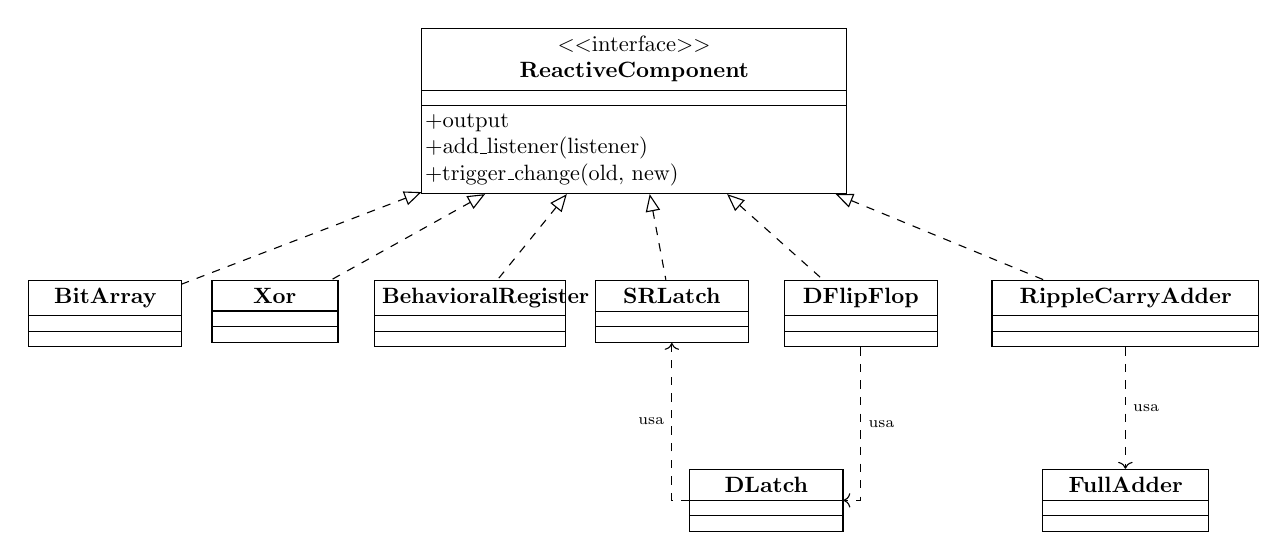
\begin{tikzpicture}[scale=0.8, every node/.style={transform shape}]
\begin{interface}[text width=6.5cm]{ReactiveComponent}{0,0}
\operation{+output}
\operation{+add\_listener(listener)}
\operation{+trigger\_change(old, new)}
\end{interface}

\begin{class}[text width=2.2cm]{BitArray}{-8.4,-4}
\implement{ReactiveComponent}
\end{class}

\begin{class}[text width=1.6cm]{Xor}{-5.7,-4}
\implement{ReactiveComponent}
\end{class}

\begin{class}[text width=2.8cm]{BehavioralRegister}{-2.6,-4}
\implement{ReactiveComponent}
\end{class}

\begin{class}[text width=2.2cm]{SRLatch}{0.6,-4}
\implement{ReactiveComponent}
\end{class}

\begin{class}[text width=2.2cm]{DFlipFlop}{3.6,-4}
\implement{ReactiveComponent}
\end{class}

\begin{class}[text width=4.0cm]{RippleCarryAdder}{7.8,-4}
\implement{ReactiveComponent}
\end{class}

\begin{class}[text width=2.2cm]{DLatch}{2.1,-7}
\end{class}

\begin{class}[text width=2.4cm]{FullAdder}{7.8,-7}
\end{class}

\draw[dashed,->] (RippleCarryAdder.south) -- (FullAdder.north) node[midway, right]{\scriptsize usa};
\draw[dashed,->] (DFlipFlop.south) |- (DLatch.east) node[pos=0.25, right]{\scriptsize usa};
\draw[dashed,->] (DLatch.west) -| (SRLatch.south) node[pos=0.75, left]{\scriptsize usa};
\end{tikzpicture}
\begin{center}
\footnotesize Fonte: elaborada pelo autor (2026).
\end{center}
\end{figure}

A Figura~\ref{fig:propagacao} ilustra essa cadeia de observadores para o circuito contador que será detalhado na Seção~\ref{sec:composicao}: cada seta indica um componente registrado como \textit{listener} de outro, e o laço inferior mostra o valor capturado pelo registrador sendo realimentado para a entrada do somador.

\begin{figure}[H]
\centering
\caption{Cadeia de propagação reativa do contador binário realimentado.}
\label{fig:propagacao}
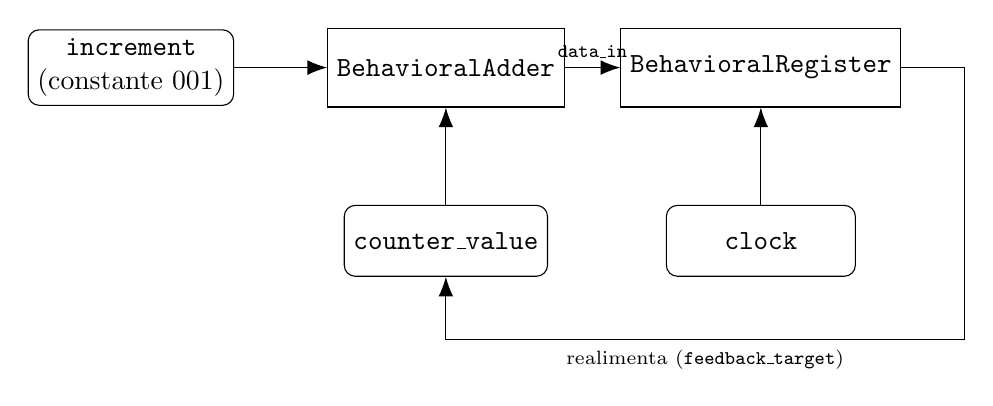
\begin{tikzpicture}[
    box/.style={draw, rectangle, minimum width=2.6cm, minimum height=1cm, align=center},
    sig/.style={draw, rectangle, rounded corners, minimum width=2.4cm, minimum height=0.9cm, align=center},
    >={Latex[length=2.5mm]}
]
    \node[sig] (const) at (0,0) {\texttt{increment}\\(constante 001)};
    \node[box] (adder) at (4,0) {\texttt{BehavioralAdder}};
    \node[box] (register) at (8,0) {\texttt{BehavioralRegister}};
    \node[sig] (value) at (4,-2.2) {\texttt{counter\_value}};
    \node[sig] (clock) at (8,-2.2) {\texttt{clock}};

    \draw[->] (const) -- (adder);
    \draw[->] (adder) -- node[above]{\scriptsize \texttt{data\_in}} (register);
    \draw[->] (value) -- (adder);
    \draw[->] (clock) -- (register);
    \draw[->] (register.east) -- ++(0.8,0) |- ($(value.south)+(0,-0.8)$) node[pos=0.75, below]{\scriptsize realimenta (\texttt{feedback\_target})} -- (value.south);
\end{tikzpicture}
\begin{center}
\footnotesize Fonte: elaborada pelo autor (2026).
\end{center}
\end{figure}

\section{Representação de Sinais}
\label{sec:sinais}

O pacote \texttt{signals} contém as três classes responsáveis por representar sinais/barramentos de \textit{bits}.

\subsection{\texttt{BitArray}}

A classe \texttt{BitArray} representa um sinal, seja ele um \textit{bit} único ou um barramento de múltiplos \textit{bits}. Em termos de circuito, um \texttt{BitArray} de um único \textit{bit} corresponde a um fio, e um \texttt{BitArray} de N \textit{bits} corresponde a um conjunto de N fios agrupados em um barramento, como ilustra a Figura~\ref{fig:fios}.

\begin{figure}[H]
\centering
\caption{Um fio (\texttt{BitArray} de 1 \textit{bit}) e um barramento de três fios (\texttt{BitArray} de 3 \textit{bits}).}
\label{fig:fios}
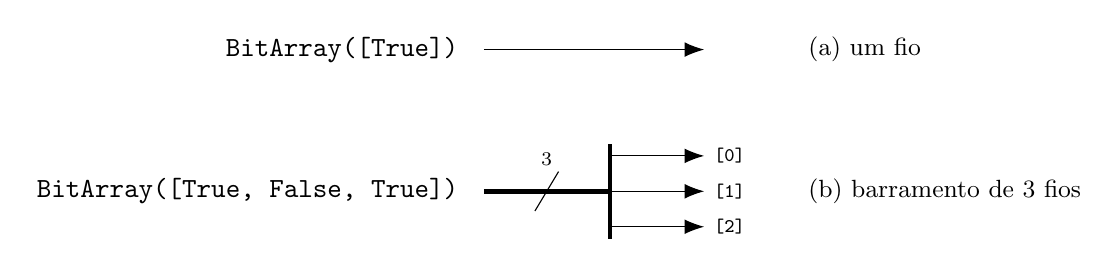
\begin{tikzpicture}[>={Latex[length=2.5mm]}]
    % (a) um fio
    \node[anchor=east] at (0,0) {\texttt{BitArray([True])}};
    \draw[->] (0.2,0) -- (3.0,0);
    \node[anchor=west] at (4.2,0) {\small (a) um fio};
    % (b) barramento de 3 fios
    \node[anchor=east] at (0,-1.8) {\texttt{BitArray([True, False, True])}};
    \draw[line width=1.6pt] (0.2,-1.8) -- (1.8,-1.8);
    \draw (0.85,-2.05) -- (1.15,-1.55);
    \node[above] at (1.0,-1.6) {\scriptsize 3};
    \draw[line width=1.6pt] (1.8,-2.4) -- (1.8,-1.2);
    \foreach \y/\t in {-1.35/[0], -1.8/[1], -2.25/[2]} {
        \draw[->] (1.8,\y) -- (3.0,\y) node[right]{\scriptsize \texttt{\t}};
    }
    \node[anchor=west] at (4.2,-1.8) {\small (b) barramento de 3 fios};
\end{tikzpicture}
\begin{center}
\footnotesize Fonte: elaborada pelo autor (2026).
\end{center}
\end{figure}

Seu construtor recebe o valor inicial, e a propriedade \texttt{output} intercepta toda atribuição para notificar os \textit{listeners} registrados, como mostra o Algoritmo~\ref{alg:bitarray}.

\begin{algoritmo}[H]
\caption{Classe BitArray (signals/bit\_array.py).}
\label{alg:bitarray}
\begin{minted}{python}
class BitArray:
    def __init__(self, initial_value):
        self._output = initial_value
        self._listeners = []

    @property
    def output(self):
        return self._output

    @output.setter
    def output(self, value):
        previous_output = self._output
        if value == previous_output:
            return
        self._output = value
        for listener in self._listeners:
            listener(previous_output, value)

    def add_listener(self, listener):
        self._listeners.append(listener)
\end{minted}
\begin{center}
\footnotesize Fonte: elaborado pelo autor (2026).
\end{center}
\end{algoritmo}

O uso do decorador \texttt{@property} (Linhas 6 e 10 do Algoritmo~\ref{alg:bitarray}) é o que torna a notificação transparente: do ponto de vista do código cliente, \texttt{sinal.output = novo\_valor} é uma simples atribuição, mas internamente ela dispara a notificação de todos os componentes conectados a esse sinal.

\subsection{\texttt{BitSlice} e \texttt{Bus}}

As portas lógicas (Seção~\ref{sec:portas}) operam elemento a elemento sobre barramentos do mesmo tamanho, mas não propagam \textit{carry} entre posições de \textit{bit}. Para montar um somador de N \textit{bits} com propagação de \textit{carry} (Seção~\ref{sec:somador-portas}), é preciso operar em cada \textit{bit} individualmente. Duas classes auxiliares resolvem esse problema:

\begin{itemize}
    \item \texttt{BitSlice(source, index)} projeta um único \textit{bit} de um sinal maior como um sinal próprio de 1 \textit{bit}, atualizando-se automaticamente quando \texttt{source} muda;
    \item \texttt{Bus(bits)} faz o caminho inverso, combinando uma lista de sinais de 1 \textit{bit} (do mais ao menos significativo) em um único sinal de N \textit{bits}.
\end{itemize}

Em termos de fios, \texttt{BitSlice} corresponde a retirar um único fio de um barramento, e \texttt{Bus} a agrupar vários fios independentes em um novo barramento, como ilustra a Figura~\ref{fig:bitslice-bus}.

\begin{figure}[H]
\centering
\caption{\texttt{BitSlice} retirando fios de um barramento e \texttt{Bus} agrupando fios em um barramento.}
\label{fig:bitslice-bus}
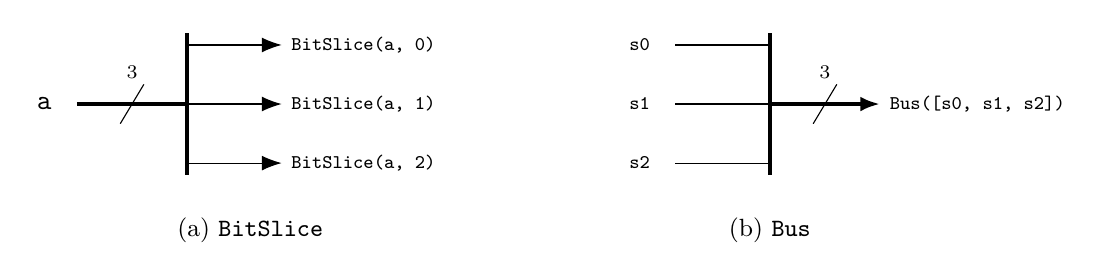
\begin{tikzpicture}[>={Latex[length=2.5mm]}]
    % (a) BitSlice
    \node[anchor=east] at (0,0) {\texttt{a}};
    \draw[line width=1.6pt] (0.2,0) -- (1.6,0);
    \draw (0.75,-0.25) -- (1.05,0.25);
    \node[above] at (0.9,0.2) {\scriptsize 3};
    \draw[line width=1.6pt] (1.6,-0.9) -- (1.6,0.9);
    \foreach \y/\i in {0.75/0, 0/1, -0.75/2} {
        \draw[->] (1.6,\y) -- (2.8,\y) node[right]{\scriptsize \texttt{BitSlice(a, \i)}};
    }
    \node at (2.4,-1.6) {\small (a) \texttt{BitSlice}};
    % (b) Bus
    \foreach \y/\i in {0.75/0, 0/1, -0.75/2} {
        \node[anchor=east] at (7.6,\y) {\scriptsize \texttt{s\i}};
        \draw (7.8,\y) -- (9,\y);
    }
    \draw[line width=1.6pt] (9,-0.9) -- (9,0.9);
    \draw[->, line width=1.6pt] (9,0) -- (10.4,0);
    \draw (9.55,-0.25) -- (9.85,0.25);
    \node[above] at (9.7,0.2) {\scriptsize 3};
    \node[right] at (10.4,0) {\scriptsize \texttt{Bus([s0, s1, s2])}};
    \node at (9,-1.6) {\small (b) \texttt{Bus}};
\end{tikzpicture}
\begin{center}
\footnotesize Fonte: elaborada pelo autor (2026).
\end{center}
\end{figure}

Ambas seguem o mesmo contrato (\texttt{output}, \texttt{add\_listener}, \texttt{trigger\_change}) e são usadas internamente pelo \texttt{RippleCarryAdder}, descrito na Seção~\ref{sec:somador-portas}.

\section{Portas Lógicas}
\label{sec:portas}

As portas lógicas (\texttt{Not}, \texttt{And}, \texttt{Or}, \texttt{Xor}, no pacote \texttt{gates}) seguem todas a mesma estrutura: recebem seus componentes de entrada no construtor, se registram como \textit{listeners} deles e calculam a saída \textit{bit} a \textit{bit}. O Algoritmo~\ref{alg:xor} apresenta, como exemplo, a porta \texttt{Xor}.

\begin{algoritmo}[H]
\caption{Porta Xor (gates/xor\_gate.py).}
\label{alg:xor}
\begin{minted}{python}
class Xor:
    def __init__(self, a, b):
        self._a = a
        self._b = b
        self._output = None
        self._listeners = []

        self._a.add_listener(self.trigger_change)
        self._b.add_listener(self.trigger_change)
        self.trigger_change(None, None)

    def trigger_change(self, old, new):
        previous_output = self._output
        new_value = [self._a.output[i] ^ self._b.output[i]
                     for i in range(len(self._a.output))]
        if new_value == previous_output:
            return self._output
        self._output = new_value
        for listener in self._listeners:
            listener(previous_output, new_value)
        return self._output

    @property
    def output(self):
        return self._output

    def add_listener(self, listener):
        self._listeners.append(listener)
\end{minted}
\begin{center}
\footnotesize Fonte: elaborado pelo autor (2026).
\end{center}
\end{algoritmo}

As demais portas (\texttt{Not}, \texttt{And}, \texttt{Or}) diferem apenas na operação booleana aplicada a cada par de \textit{bits} das entradas (Linha 14 do Algoritmo~\ref{alg:xor}). Como cada porta se inscreve como \textit{listener} de suas entradas já no construtor (Linhas 8 e 9 do Algoritmo~\ref{alg:xor}), a saída de uma porta é recalculada automaticamente sempre que qualquer uma de suas entradas muda, sem que o código cliente precise chamar nenhum método explicitamente. A Figura~\ref{fig:xor-codigo} relaciona cada parte do símbolo da porta às linhas do Algoritmo~\ref{alg:xor} que a implementam.

\begin{figure}[H]
\centering
\caption{Porta XOR anotada com as linhas do Algoritmo~\ref{alg:xor}.}
\label{fig:xor-codigo}
\begin{circuitikz}[>={Latex[length=2mm]}]
\node[xor port] (x) at (0,0) {};
\draw (x.in 1) -- ++(-1.4,0) node[left]{\texttt{a}};
\draw (x.in 2) -- ++(-1.4,0) node[left]{\texttt{b}};
\draw (x.out) -- ++(1.6,0) node[right]{\texttt{output}};
\node[font=\scriptsize, align=left, anchor=east] (n1) at (-1.6,1.3) {L8--9: inscreve-se como\\\textit{listener} de \texttt{a} e \texttt{b}};
\draw[dashed,->] (n1.east) -- ($(x.in 1)+(-0.8,0.05)$);
\node[font=\scriptsize, align=center] (n2) at (0,-1.4) {L14--15: \texttt{a[i] \textasciicircum{} b[i]} para cada \textit{bit}; L16--17: para se nada mudou};
\draw[dashed,->] (n2.north) -- (x.south);
\node[font=\scriptsize, align=left, anchor=west] (n3) at (1.6,1.3) {L18: guarda a nova saída\\L19--20: notifica os \textit{listeners}};
\draw[dashed,->] (n3.west) -- ($(x.out)+(0.8,0.05)$);
\end{circuitikz}
\begin{center}
\footnotesize Fonte: elaborada pelo autor (2026).
\end{center}
\end{figure}

\section{Somador com Portas Lógicas}
\label{sec:somador-portas}

Esta é a forma recomendada de montar um somador no simulador: inteiramente a partir das portas lógicas básicas, sem nenhum atalho em Python. Um somador completo de 1 \textit{bit} é montado com dois meios-somadores mais uma porta OR para combinar os dois possíveis \textit{carries}, como mostra o Algoritmo~\ref{alg:fulladder}.

\begin{algoritmo}[H]
\caption{FullAdder (components/full\_adder.py).}
\label{alg:fulladder}
\begin{minted}{python}
from gates.xor_gate import Xor
from gates.and_gate import And
from gates.or_gate import Or


class FullAdder:
    def __init__(self, a, b, carry_in):
        xor_ab = Xor(a, b)
        and_ab = And(a, b)
        and_xor_carry = And(xor_ab, carry_in)

        self.sum = Xor(xor_ab, carry_in)
        self.carry_out = Or(and_ab, and_xor_carry)
\end{minted}
\begin{center}
\footnotesize Fonte: elaborado pelo autor (2026).
\end{center}
\end{algoritmo}

A Figura~\ref{fig:full-adder} mostra o mesmo circuito representado com os símbolos de portas lógicas apresentados na Seção~\ref{sec:circuitos-digitais}, evidenciando a correspondência direta entre o diagrama e o código: cada porta lógica do diagrama corresponde a uma instância de \texttt{Xor}, \texttt{And} ou \texttt{Or} no construtor de \texttt{FullAdder}, e está anotada com a linha do Algoritmo~\ref{alg:fulladder} que a cria.

\begin{figure}[H]
\centering
\caption{Somador completo (\textit{full adder}) montado com portas lógicas, com a linha do Algoritmo~\ref{alg:fulladder} correspondente a cada porta.}
\label{fig:full-adder}
\begin{circuitikz}[scale=0.9, every node/.style={transform shape}]
\node[xor port] (x1) at (2.4,0) {};
\node[and port] (a1) at (2.4,-3.2) {};
\node[xor port, anchor=in 1] (x2) at (5.6,0) {};
\node[and port, anchor=in 1] (a2) at (5.6,-1.6) {};
\node[or port] (o1) at (10.6,-2.4) {};

% entradas A e B
\draw (-0.4,0 |- x1.in 1) node[left]{$A$} -- (x1.in 1);
\draw (-0.4,0 |- x1.in 2) node[left]{$B$} -- (x1.in 2);
\draw (0.6,0 |- x1.in 1) node[circ]{} |- (a1.in 1);
\draw (0.1,0 |- x1.in 2) node[circ]{} |- (a1.in 2);

% Cin
\draw (-0.4,0 |- a2.in 2) node[left]{$C_{in}$} -- (4.9,0 |- a2.in 2) node[circ]{} -- (a2.in 2);
\draw (4.9,0 |- a2.in 2) |- (x2.in 2);

% saída de xor_ab alimenta xor2 e and2
\draw (x1.out) -- (x2.in 1);
\draw (4.4,0 |- x1.out) node[circ]{} |- (a2.in 1);

% carries para a porta OR
\draw (a2.out) -| (9.0,0 |- o1.in 1) -- (o1.in 1);
\draw (a1.out) -| (9.0,0 |- o1.in 2) -- (o1.in 2);

% saídas
\draw (x2.out) -- ++(1.2,0) node[right]{Soma};
\draw (o1.out) -- ++(0.6,0) node[right]{\textit{Carry-out}};

% linhas do código
\node[font=\scriptsize, above=2mm] at (x1.north) {L8: \texttt{xor\_ab}};
\node[font=\scriptsize, below=2mm] at (a1.south) {L9: \texttt{and\_ab}};
\node[font=\scriptsize, above=2mm] at (x2.north) {L12: \texttt{self.sum}};
\node[font=\scriptsize, below=1mm] at (a2.south) {L10: \texttt{and\_xor\_carry}};
\node[font=\scriptsize, below=2mm] at (o1.south) {L13: \texttt{self.carry\_out}};
\end{circuitikz}
\begin{center}
\footnotesize Fonte: elaborada pelo autor (2026).
\end{center}
\end{figure}

\texttt{FullAdder} expõe \texttt{.sum} e \texttt{.carry\_out} como saídas de portas lógicas comuns (Linhas 12 e 13 do Algoritmo~\ref{alg:fulladder}), prontas para servir de entrada a outro componente. O \texttt{RippleCarryAdder}, apresentado no Algoritmo~\ref{alg:rca}, encadeia N instâncias de \texttt{FullAdder}, uma por \textit{bit}, do menos significativo ao mais significativo, usando \texttt{BitSlice} para extrair cada \textit{bit} dos barramentos de entrada e um \texttt{Bus} para recompor os N \textit{bits} de soma em um único sinal.

\begin{algoritmo}[H]
\caption{RippleCarryAdder (components/ripple\_carry\_adder.py).}
\label{alg:rca}
\begin{minted}{python}
class RippleCarryAdder:
    def __init__(self, a, b, carry_in=None):
        width = len(a.output)
        carry = carry_in if carry_in is not None else BitArray([False])

        sum_bits = [None] * width
        self.full_adders = []
        for i in range(width - 1, -1, -1):
            bit_a = BitSlice(a, i)
            bit_b = BitSlice(b, i)
            full_adder = FullAdder(bit_a, bit_b, carry)
            self.full_adders.append(full_adder)
            sum_bits[i] = full_adder.sum
            carry = full_adder.carry_out

        self.sum = Bus(sum_bits)
        self.carry_out = carry
\end{minted}
\begin{center}
\footnotesize Fonte: elaborado pelo autor (2026).
\end{center}
\end{algoritmo}

A Figura~\ref{fig:rca} mostra a estrutura resultante para N = 3, anotada com as linhas do código: o laço das Linhas 8 a 14 do Algoritmo~\ref{alg:rca} percorre os \textit{bits} do menos significativo (índice 2, à direita) ao mais significativo (índice 0, à esquerda), e a variável \texttt{carry} (Linha 14) conecta o \textit{carry-out} de cada \texttt{FullAdder} ao \textit{carry-in} do seguinte. A lista \texttt{full\_adders} (Linhas 7 e 12) não participa da soma: ela apenas guarda os estágios criados, para que possam ser inspecionados depois da construção (Seção~\ref{sec:observacao}).

\begin{figure}[H]
\centering
\caption{\texttt{RippleCarryAdder} de 3 \textit{bits} formado pelo encadeamento de três \texttt{FullAdder}, com as linhas do Algoritmo~\ref{alg:rca}.}
\label{fig:rca}
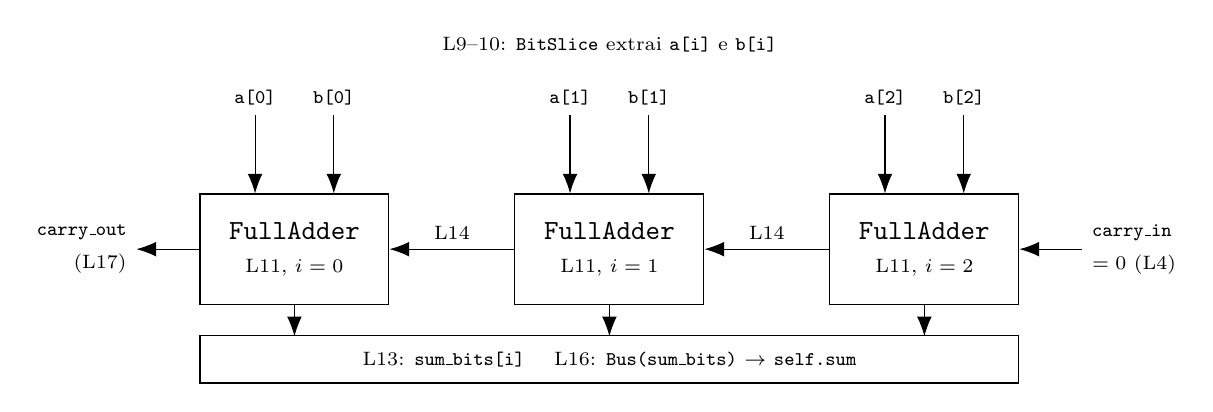
\begin{tikzpicture}[
    fa/.style={draw, rectangle, minimum width=2.4cm, minimum height=1.4cm, align=center},
    >={Latex[length=2.5mm]}
]
    \foreach \i/\x in {0/0, 1/4, 2/8} {
        \node[fa] (fa\i) at (\x,0) {\texttt{FullAdder}\\\scriptsize L11, $i = \i$};
        \draw[<-] ($(fa\i.north)+(-0.5,0)$) -- ++(0,1) node[above]{\scriptsize \texttt{a[\i]}};
        \draw[<-] ($(fa\i.north)+(0.5,0)$) -- ++(0,1) node[above]{\scriptsize \texttt{b[\i]}};
        \draw[->] (fa\i.south) -- ++(0,-0.4);
    }
    \node[font=\scriptsize] at (4,2.6) {L9--10: \texttt{BitSlice} extrai \texttt{a[i]} e \texttt{b[i]}};
    \node[draw, minimum width=10.4cm, minimum height=0.6cm, font=\scriptsize] (bus) at (4,-1.4) {L13: \texttt{sum\_bits[i]} \quad L16: \texttt{Bus(sum\_bits)} $\rightarrow$ \texttt{self.sum}};
    \draw[<-] (fa2.east) -- ++(0.8,0) node[right, align=left]{\scriptsize \texttt{carry\_in}\\\scriptsize $= 0$ (L4)};
    \draw[->] (fa2.west) -- node[above]{\scriptsize L14} (fa1.east);
    \draw[->] (fa1.west) -- node[above]{\scriptsize L14} (fa0.east);
    \draw[->] (fa0.west) -- ++(-0.8,0) node[left, align=right]{\scriptsize \texttt{carry\_out}\\\scriptsize (L17)};
\end{tikzpicture}
\begin{center}
\footnotesize Fonte: elaborada pelo autor (2026).
\end{center}
\end{figure}

Um ponto central deste trabalho é que, aqui, o \textit{overflow} não é tratado por nenhuma função de \textit{padding} ou truncamento: ele surge naturalmente da topologia do circuito. A soma só tem $N$ fios de saída, um por estágio de \texttt{FullAdder}, e o ``vai-um'' do último estágio vira um sinal \texttt{carry\_out} separado. Quando esse sinal não é conectado a mais nada, a informação do estouro se perde e a soma ``dá a volta'' sozinha, exatamente como aconteceria em um contador de \textit{hardware} real. Esse comportamento é validado e discutido em detalhe na Seção~\ref{sec:contador-portas}.

\section{\texttt{BehavioralAdder}: um Somador Comportamental em Python}
\label{sec:behavioral-adder}

O pacote \texttt{components} também inclui o \texttt{BehavioralAdder}, apresentado no Algoritmo~\ref{alg:behavioraladder}, que soma dois \texttt{BitArray} sem montar nenhuma porta lógica: ele segue o mesmo contrato reativo das portas, mas, em vez de uma operação booleana, delega o cálculo da saída (Linha 14) à função \texttt{sum\_via\_integer\_conversion}.

\begin{algoritmo}[H]
\caption{BehavioralAdder (components/behavioral\_adder.py).}
\label{alg:behavioraladder}
\begin{minted}{python}
class BehavioralAdder:
    def __init__(self, a, b):
        self._a = a
        self._b = b
        self._output = None
        self._listeners = []

        self._a.add_listener(self.trigger_change)
        self._b.add_listener(self.trigger_change)
        self.trigger_change(None, None)

    def trigger_change(self, old, new):
        previous_output = self._output
        new_value = sum_via_integer_conversion(self._a.output, self._b.output)
        if new_value == previous_output:
            return self._output
        self._output = new_value
        for listener in self._listeners:
            listener(previous_output, new_value)
        return self._output

    @property
    def output(self):
        return self._output

    def add_listener(self, listener):
        self._listeners.append(listener)
\end{minted}
\begin{center}
\footnotesize Fonte: elaborado pelo autor (2026).
\end{center}
\end{algoritmo}

As funções auxiliares usadas pelo \texttt{BehavioralAdder} estão no módulo \texttt{utils/binary\_conversion.py}, apresentado no Algoritmo~\ref{alg:binconv}: \texttt{sum\_via\_integer\_conversion} (Linhas 1--6) converte as duas entradas para inteiro com \texttt{binary\_array\_to\_int} (Linhas 9--11), soma os inteiros em Python, converte o resultado de volta para uma lista de \textit{bits} com \texttt{int\_to\_binary\_array} (Linhas 14--16) e, por fim, ajusta essa lista ao tamanho da entrada com \texttt{pad\_binary\_array} (Linhas 19--24).

\begin{algoritmo}[H]
\caption{Funções auxiliares de conversão e \textit{padding} binário (utils/binary\_conversion.py).}
\label{alg:binconv}
\begin{minted}{python}
def sum_via_integer_conversion(a, b):
    a_int = binary_array_to_int(a)
    b_int = binary_array_to_int(b)
    sum_int = a_int + b_int
    sum_array = int_to_binary_array(sum_int)
    return pad_binary_array(sum_array, len(a))


def binary_array_to_int(binary_array):
    bits_as_str = "".join("1" if bit else "0" for bit in binary_array)
    return int(bits_as_str, 2)


def int_to_binary_array(value):
    binary_str = bin(value)[2:]
    return [bit == "1" for bit in binary_str]


def pad_binary_array(binary_array, length):
    if len(binary_array) < length:
        return [False] * (length - len(binary_array)) + binary_array
    if len(binary_array) > length:
        return binary_array[-length:]
    return binary_array[:]
\end{minted}
\begin{center}
\footnotesize Fonte: elaborado pelo autor (2026).
\end{center}
\end{algoritmo}

Como o nome indica, trata-se de uma \textbf{descrição comportamental} do somador, no mesmo sentido usado nas HDLs (Seção~\ref{sec:hdls}): o componente descreve o que o somador faz, e não de quais portas ele é feito, como ocorre na descrição estrutural do \texttt{RippleCarryAdder}. Não se trata, portanto, de uma tentativa imperfeita de somador digital, e sim de uma abstração deliberada: um recurso do simulador que demonstra a possibilidade de \textbf{misturar um trecho de Python ``puro'' com o restante do circuito reativo}. Isso é útil quando o objetivo de um teste ou demonstração é outra parte do circuito, por exemplo, o comportamento do registrador e da realimentação de um contador, e não a aritmética em si. Nesses casos, o \texttt{BehavioralAdder} permite ao estudante montar rapidamente um circuito funcional sem precisar implementar previamente um somador com portas lógicas, substituindo-o pelo \texttt{RippleCarryAdder} (Seção~\ref{sec:somador-portas}) somente quando o próprio somador for o objeto de estudo.

A Figura~\ref{fig:behavioral-adder} representa o \texttt{BehavioralAdder} como um bloco: externamente, ele tem as mesmas entradas e a mesma saída de um somador de portas lógicas; internamente, em vez de portas interligadas (como na Figura~\ref{fig:rca}), há apenas uma sequência de operações em Python, cada uma anotada com as linhas dos Algoritmos~\ref{alg:behavioraladder} e~\ref{alg:binconv} que a implementam.

\begin{figure}[H]
\centering
\caption{\texttt{BehavioralAdder} como bloco comportamental, com as linhas dos Algoritmos~\ref{alg:behavioraladder} e~\ref{alg:binconv}.}
\label{fig:behavioral-adder}
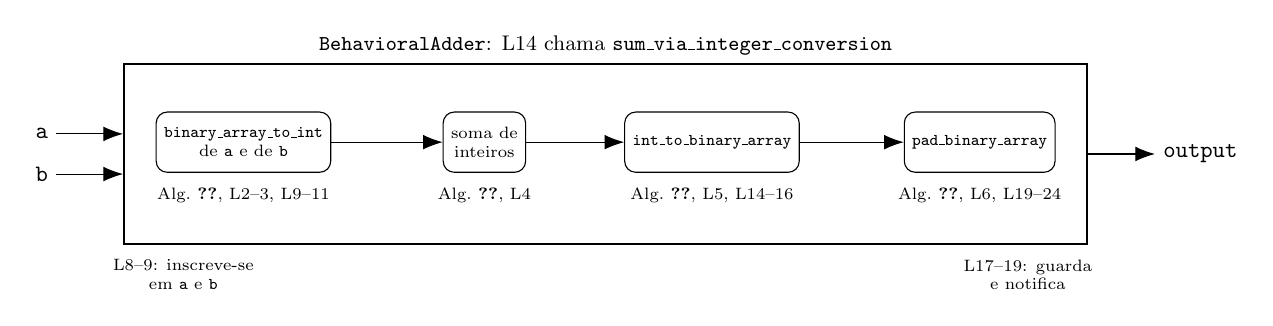
\begin{tikzpicture}[
    etapa/.style={draw, rounded corners, font=\scriptsize, align=center, minimum height=0.9cm},
    >={Latex[length=2.5mm]}, scale=0.85, every node/.style={transform shape}
]
    \node[etapa] (s1) at (0,0) {\texttt{binary\_array\_to\_int}\\de \texttt{a} e de \texttt{b}};
    \node[etapa] (s2) at (3.6,0) {soma de\\inteiros};
    \node[etapa] (s3) at (7.0,0) {\texttt{int\_to\_binary\_array}};
    \node[etapa] (s4) at (11.0,0) {\texttt{pad\_binary\_array}};
    \draw[->] (s1) -- (s2);
    \draw[->] (s2) -- (s3);
    \draw[->] (s3) -- (s4);
    \node[font=\scriptsize, below=1mm of s1] {Alg.~\ref{alg:binconv}, L2--3, L9--11};
    \node[font=\scriptsize, below=1mm of s2] {Alg.~\ref{alg:binconv}, L4};
    \node[font=\scriptsize, below=1mm of s3] {Alg.~\ref{alg:binconv}, L5, L14--16};
    \node[font=\scriptsize, below=1mm of s4] {Alg.~\ref{alg:binconv}, L6, L19--24};
    \node[draw, thick, fit=(s1) (s4), inner xsep=0.4cm, inner ysep=0.75cm, yshift=-0.15cm] (box) {};
    \node[font=\small, anchor=south] at (box.north) {\texttt{BehavioralAdder}: L14 chama \texttt{sum\_via\_integer\_conversion}};
    \draw[<-] ($(box.west)+(0,0.3)$) -- ++(-1,0) node[left]{\texttt{a}};
    \draw[<-] ($(box.west)+(0,-0.3)$) -- ++(-1,0) node[left]{\texttt{b}};
    \draw[->] (box.east) -- ++(1,0) node[right]{\texttt{output}};
    \node[font=\scriptsize, align=center, anchor=north] at ($(box.south west)+(0.9,-0.1)$) {L8--9: inscreve-se\\em \texttt{a} e \texttt{b}};
    \node[font=\scriptsize, align=center, anchor=north] at ($(box.south east)+(-0.9,-0.1)$) {L17--19: guarda\\e notifica};
\end{tikzpicture}
\begin{center}
\footnotesize Fonte: elaborada pelo autor (2026).
\end{center}
\end{figure}

A função \texttt{pad\_binary\_array} merece destaque: ela garante que o resultado da soma tenha exatamente o mesmo número de \textit{bits} da entrada original, preenchendo com zeros à esquerda quando o resultado é menor (Linhas 20 e 21 do Algoritmo~\ref{alg:binconv}), e \textbf{truncando os \textit{bits} mais significativos} quando o resultado excede esse tamanho (Linhas 22 e 23), o que reproduz o \textit{overflow} apenas dentro da descrição comportamental do \texttt{BehavioralAdder}. É importante notar que essa função é usada exclusivamente por \texttt{sum\_via\_integer\_conversion}: quando o somador é montado com portas lógicas (\texttt{RippleCarryAdder}), como discutido na Seção~\ref{sec:somador-portas}, o \textit{overflow} é tratado de forma completamente diferente, pelo sinal \texttt{carry\_out}, e \texttt{pad\_binary\_array} não entra em jogo.

O truncamento das Linhas 22 e 23 não existia na primeira versão da função, que apenas preenchia o resultado com zeros à esquerda. Ao executar o contador de 3 \textit{bits} com \texttt{BehavioralAdder} além do valor \texttt{111}, o oitavo pulso de \textit{clock} produzia \texttt{[True, False, False, False]}: em vez de voltar a \texttt{000}, como um contador real, o contador crescia em largura. O episódio ilustra que a propagação automática de valores garante que os componentes sejam recalculados na ordem correta, mas não que cada componente reproduza fielmente o comportamento do \textit{hardware}; essa fidelidade precisa ser verificada componente a componente, sobretudo nas descrições comportamentais, em que a lógica é escrita livremente em Python.

\section{Componente Sequencial: \texttt{BehavioralRegister}}
\label{sec:register}

O \texttt{BehavioralRegister} é o componente do simulador com comportamento sensível a borda de \textit{clock} mais simples de usar, e é o que dá início aos circuitos sequenciais: qualquer circuito com estado (contador, \textit{flip-flop}) depende de um registrador para ``lembrar'' um valor entre pulsos de \textit{clock}. É importante ser explícito sobre sua natureza, que o próprio nome indica, assim como no \texttt{BehavioralAdder}: o \texttt{BehavioralRegister} é uma \textbf{descrição comportamental em lógica Python}, não um circuito montado a partir de portas lógicas; sua contraparte estrutural é o \texttt{DFlipFlopRegister} (Seção~\ref{sec:dflipflop-register}). Ele não modela o funcionamento interno de um \textit{flip-flop} real (não há \textit{latches}, não há a estrutura mestre-escravo discutida na Seção~\ref{sec:latches}); ele apenas verifica, em Python, se o \textit{clock} transicionou de falso para verdadeiro e, em caso afirmativo, lê diretamente o valor atual de sua entrada. Ele recebe um sinal \texttt{clock}, um componente \texttt{data\_in} (o dado a ser capturado) e, opcionalmente, um componente \texttt{feedback\_target} a ser notificado quando o registrador atualizar seu valor, como mostra o Algoritmo~\ref{alg:register}.

\begin{algoritmo}[H]
\caption{Classe BehavioralRegister (components/behavioral\_register.py).}
\label{alg:register}
\begin{minted}{python}
def _is_high(value):
    if isinstance(value, list):
        return bool(value) and bool(value[0])
    return bool(value)


class BehavioralRegister:
    def __init__(self, clock, data_in, feedback_target=None):
        self._clock = clock
        self._data_in = data_in
        self._output = None
        self._listeners = []

        self._clock.add_listener(self.trigger_change)
        if feedback_target is not None:
            self.add_listener(feedback_target.trigger_change)

    def trigger_change(self, old, new):
        previous_output = self._output
        if not _is_high(old) and _is_high(new):
            self._output = self._data_in.output
            for listener in self._listeners:
                listener(previous_output, self._output)
        return self._output

    @property
    def output(self):
        return self._output

    def add_listener(self, listener):
        self._listeners.append(listener)
\end{minted}
\begin{center}
\footnotesize Fonte: elaborado pelo autor (2026).
\end{center}
\end{algoritmo}

O condicional da Linha 20 do Algoritmo~\ref{alg:register} é o que implementa a detecção de borda de subida: o valor de \texttt{data\_in.output} só é capturado quando \texttt{clock.output} muda de falso para verdadeiro. A função auxiliar \texttt{\_is\_high} (Linhas 1--4) existe porque o \textit{clock} pode ser representado tanto por um booleano (\texttt{BitArray(False)}) quanto por uma lista de um único \textit{bit} (\texttt{BitArray([False])}), forma exigida quando o mesmo sinal também alimenta portas lógicas (Seção~\ref{sec:contador-registrador-real}). Em Python, qualquer lista não vazia é considerada verdadeira, inclusive \texttt{[False]}; uma versão anterior deste componente testava apenas a ``veracidade'' do novo valor e, com um \textit{clock} em forma de lista, capturava o dado também na borda de descida. Esse defeito foi identificado durante a revisão do trabalho e passou a ser coberto por um teste automatizado (Seção~\ref{sec:testes}). Para gerar um pulso de \textit{clock}, é necessário alternar explicitamente o valor do \textit{clock} entre falso e verdadeiro (\texttt{clock.output = False} seguido de \texttt{clock.output = True}); atribuir verdadeiro repetidamente, sem antes voltar a falso, não gera uma nova borda e, portanto, não atualiza o registrador.

O parâmetro opcional \texttt{feedback\_target} (Linhas 15 e 16) é o que permite fechar um laço de realimentação: ao passar o próprio sinal de entrada de um circuito como \texttt{feedback\_target} do registrador, o valor atualizado do registrador é propagado de volta para esse sinal, fazendo com que o circuito combinacional ligado a ele seja recalculado antes do próximo pulso de \textit{clock}. Esse mecanismo é a base dos circuitos com estado apresentados a seguir. A Figura~\ref{fig:behavioral-register} representa o \texttt{BehavioralRegister} com o símbolo usual de um registrador e indica as linhas do Algoritmo~\ref{alg:register} responsáveis por cada parte; no lugar dos \textit{latches} internos de um registrador real (Seção~\ref{sec:latches}), há apenas um condicional em Python.

\begin{figure}[H]
\centering
\caption{\texttt{BehavioralRegister} representado como registrador, com as linhas do Algoritmo~\ref{alg:register}.}
\label{fig:behavioral-register}
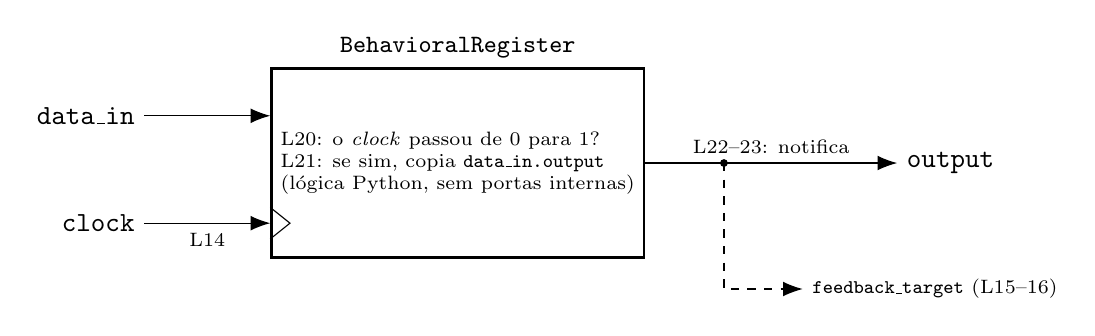
\begin{tikzpicture}[>={Latex[length=2.5mm]}]
    \node[draw, thick, minimum width=4.6cm, minimum height=2.4cm, align=left, font=\scriptsize] (r) at (0,0) {L20: o \textit{clock} passou de 0 para 1?\\L21: se sim, copia \texttt{data\_in.output}\\(lógica Python, sem portas internas)};
    \node[font=\small, anchor=south] at (r.north) {\texttt{BehavioralRegister}};
    \draw ($(r.south west)+(0,0.25)$) -- ++(0.25,0.2) -- ++(-0.25,0.2);
    \draw[<-] ($(r.west)+(0,0.6)$) -- ++(-1.6,0) node[left]{\texttt{data\_in}};
    \draw[<-] ($(r.south west)+(0,0.45)$) -- ++(-1.6,0) node[left]{\texttt{clock}} node[pos=0.5, below, font=\scriptsize]{L14};
    \draw[->] (r.east) -- ++(3.2,0) node[right]{\texttt{output}} node[pos=0.5, above, font=\scriptsize]{L22--23: notifica};
    \node[font=\scriptsize, anchor=west] (fb) at ($(r.east)+(2.0,-1.6)$) {\texttt{feedback\_target} (L15--16)};
    \draw[->, dashed] ($(r.east)+(1.0,0)$) node[circle, fill, inner sep=1pt]{} |- (fb.west);
\end{tikzpicture}
\begin{center}
\footnotesize Fonte: elaborada pelo autor (2026).
\end{center}
\end{figure}

\section{Registrador Real com \textit{Latches}}
\label{sec:latches}

Como discutido na Seção~\ref{sec:register}, o \texttt{BehavioralRegister} é uma abstração. Para complementá-lo com uma implementação que reproduz de fato a estrutura interna de um \textit{flip-flop}, o pacote \texttt{components} também inclui um registrador construído inteiramente a partir de portas lógicas, em três camadas: um \textbf{\textit{latch} SR}, um \textbf{\textit{latch} D} e um \textbf{\textit{flip-flop} D mestre-escravo}.

\subsection{\textit{Latch} SR}

O \textit{latch} SR é o elemento de memória mais simples: duas portas NOR cruzadas, em que a saída de cada uma alimenta a entrada da outra. Essa realimentação combinacional genuína (a saída $Q$ depende de $\overline{Q}$, que depende de $Q$) não pode ser expressa com a ordem de construção usual dos demais componentes deste trabalho, em que cada objeto recebe suas entradas já prontas no construtor: aqui, no momento em que a primeira porta NOR precisa ser criada, a segunda ainda não existe. A solução adotada, apresentada no Algoritmo~\ref{alg:srlatch}, usa um \texttt{BitArray} comum como sinal provisório (um ``proxy''), montado antes das duas portas NOR (Linha 7) e sincronizado ao valor real assim que ambas existem (Linhas 12 e 13).

\begin{algoritmo}[H]
\caption{SRLatch (components/sr\_latch.py).}
\label{alg:srlatch}
\begin{minted}{python}
from signals.bit_array import BitArray
from gates.nor_gate import Nor


class SRLatch:
    def __init__(self, s, r):
        q_not_proxy = BitArray([False])

        self.q = Nor(r, q_not_proxy)
        self.q_not = Nor(s, self.q)

        self.q_not.add_listener(q_not_proxy.trigger_change)
        q_not_proxy.output = self.q_not.output
\end{minted}
\begin{center}
\footnotesize Fonte: elaborado pelo autor (2026).
\end{center}
\end{algoritmo}

A Figura~\ref{fig:srlatch} mostra o mesmo circuito com o símbolo das duas portas NOR: a porta superior corresponde à Linha 9 do Algoritmo~\ref{alg:srlatch}, a inferior à Linha 10, e o fio de realimentação de $\overline{Q}$ para a porta superior passa pelo \textit{proxy} criado na Linha 7 e sincronizado nas Linhas 12 e 13.

\begin{figure}[H]
\centering
\caption{\textit{Latch} SR de portas NOR cruzadas, com as linhas do Algoritmo~\ref{alg:srlatch}.}
\label{fig:srlatch}
\begin{circuitikz}
\node[nor port] (n1) at (3,1.6) {};
\node[nor port] (n2) at (3,-1.6) {};
\draw (n1.in 1) -- ++(-1.8,0) node[left]{$R$ (\texttt{r})};
\draw (n2.in 2) -- ++(-1.8,0) node[left]{$S$ (\texttt{s})};
\draw (n1.out) -- ++(1.8,0) node[right]{$Q$ (\texttt{self.q})};
\draw (n2.out) -- ++(1.8,0) node[right]{$\overline{Q}$ (\texttt{self.q\_not})};
\coordinate (qtap) at ($(n1.out)+(0.5,0)$);
\coordinate (qntap) at ($(n2.out)+(1.0,0)$);
\coordinate (qleft) at ($(n2.in 1)+(-0.4,0)$);
\coordinate (qnleft) at ($(n1.in 2)+(-0.8,0)$);
\draw (qtap) node[circ]{} |- (qleft |- 0,-0.5) |- (n2.in 1);
\draw (qntap) node[circ]{} |- (qnleft |- 0,0.5) |- (n1.in 2);
\node[draw, fill=white, font=\scriptsize] at (3,0.5) {\texttt{q\_not\_proxy} (L7)};
\node[font=\scriptsize, above=1mm] at (n1.north) {L9: \texttt{Nor(r, q\_not\_proxy)}};
\node[font=\scriptsize, below=1mm] at (n2.south) {L10: \texttt{Nor(s, self.q)}};
\node[font=\scriptsize, align=left, anchor=west] at ($(qntap)+(0.15,1.3)$) {L12--13: $\overline{Q}$\\atualiza o \textit{proxy}};
\end{circuitikz}
\begin{center}
\footnotesize Fonte: elaborada pelo autor (2026).
\end{center}
\end{figure}

Esse laço de realimentação só funciona porque as portas lógicas do simulador (Seção~\ref{sec:portas}) foram ajustadas para notificar seus \textit{listeners} apenas quando o valor calculado realmente muda; sem essa condição, a notificação de uma mudança em $Q$ dispararia uma nova notificação em $\overline{Q}$, que dispararia outra em $Q$, indefinidamente. A Seção~\ref{sec:contador-portas-real} discute o que acontece quando essa condição de parada, sozinha, não é suficiente.

\subsection{\textit{Latch} D e \textit{Flip-Flop} D Mestre-Escravo}

Um \textit{latch} D elimina a combinação inválida do \textit{latch} SR ($S = R = 1$) derivando $S$ e $R$ de um único sinal de dado $D$ e de um sinal de habilitação (\textit{enable}): $S = D \land \mathit{enable}$ e $R = \overline{D} \land \mathit{enable}$, de modo que $S$ e $R$ nunca são verdadeiros ao mesmo tempo. Enquanto \textit{enable} está em nível alto, o \textit{latch} é transparente e acompanha $D$; quando \textit{enable} cai, ele retém o último valor observado. O Algoritmo~\ref{alg:dlatch} implementa essas expressões nas Linhas 8 a 10.

\begin{algoritmo}[H]
\caption{DLatch (components/d\_latch.py).}
\label{alg:dlatch}
\begin{minted}{python}
from gates.and_gate import And
from gates.not_gate import Not
from components.sr_latch import SRLatch


class DLatch:
    def __init__(self, d, enable):
        not_d = Not(d)
        s = And(d, enable)
        r = And(not_d, enable)

        self._sr_latch = SRLatch(s, r)

    @property
    def output(self):
        return self._sr_latch.output

    def add_listener(self, listener):
        self._sr_latch.add_listener(listener)
\end{minted}
\begin{center}
\footnotesize Fonte: elaborado pelo autor (2026).
\end{center}
\end{algoritmo}

A Figura~\ref{fig:dlatch} mostra a estrutura correspondente: a porta NOT e as duas portas AND, criadas nas Linhas 8 a 10 do Algoritmo~\ref{alg:dlatch}, geram $S$ e $R$, que alimentam o \textit{latch} SR criado na Linha 12.

\begin{figure}[H]
\centering
\caption{\textit{Latch} D montado sobre um \textit{latch} SR, com as linhas do Algoritmo~\ref{alg:dlatch}.}
\label{fig:dlatch}
\begin{circuitikz}
\node[and port] (as) at (3.4,1.1) {};
\node[and port] (ar) at (3.4,-1.1) {};
\node[not port, anchor=out] (nd) at ($(ar.in 1)+(-0.5,0)$) {};
\draw (nd.out) -- (ar.in 1);
\draw (-0.6,0 |- as.in 1) node[left]{$D$ (\texttt{d})} -- (as.in 1);
\draw (0.0,0 |- as.in 1) node[circ]{} |- (nd.in);
\draw (-0.6,0) node[left]{\textit{enable}} -- (1.9,0) node[circ]{};
\draw (1.9,0) |- (as.in 2);
\draw (1.9,0) |- (ar.in 2);
\node[draw, minimum width=1.9cm, minimum height=3.0cm, align=center] (sr) at (6.6,0) {\texttt{SRLatch}\\(L12)};
\draw (as.out) -- (sr.west |- as.out) node[right, font=\scriptsize]{$S$};
\draw (ar.out) -- (sr.west |- ar.out) node[right, font=\scriptsize]{$R$};
\draw (sr.east) -- ++(1,0) node[right]{$Q$};
\node[font=\scriptsize, above=1mm] at (as.north) {L9: \texttt{s = And(d, enable)}};
\node[font=\scriptsize, below=1mm, anchor=north west] at ($(ar.south)+(-0.4,0)$) {L10: \texttt{r = And(not\_d, enable)}};
\node[font=\scriptsize, below=1mm, anchor=north east] at ($(nd.south)+(0.3,0)$) {L8: \texttt{not\_d}};
\end{circuitikz}
\begin{center}
\footnotesize Fonte: elaborada pelo autor (2026).
\end{center}
\end{figure}

O \texttt{DFlipFlop}, apresentado no Algoritmo~\ref{alg:dflipflop}, encadeia dois \textit{latches} D em uma estrutura mestre-escravo clássica: o \textit{latch} mestre fica transparente enquanto o \textit{clock} está em nível baixo (\textit{enable} $= \overline{\mathit{clock}}$, Linha 9), acompanhando $D$; o \textit{latch} escravo fica transparente enquanto o \textit{clock} está em nível alto (\textit{enable} $= \mathit{clock}$, Linha 10), repassando o valor já congelado pelo mestre. O efeito resultante é que a saída só muda no instante da borda de subida do \textit{clock}, reproduzindo o mesmo comportamento observável do \texttt{BehavioralRegister}, mas a partir de portas lógicas reais.

\begin{algoritmo}[H]
\caption{DFlipFlop (components/d\_flip\_flop.py).}
\label{alg:dflipflop}
\begin{minted}{python}
from gates.not_gate import Not
from components.d_latch import DLatch


class DFlipFlop:
    def __init__(self, d, clock, feedback_target=None):
        not_clock = Not(clock)

        self._master = DLatch(d, not_clock)
        self._slave = DLatch(self._master, clock)

        if feedback_target is not None:
            self._slave.add_listener(feedback_target.trigger_change)
            feedback_target.trigger_change(feedback_target.output, self._slave.output)

    @property
    def output(self):
        return self._slave.output

    def add_listener(self, listener):
        self._slave.add_listener(listener)
\end{minted}
\begin{center}
\footnotesize Fonte: elaborado pelo autor (2026).
\end{center}
\end{algoritmo}

A sincronização explícita de \texttt{feedback\_target} nas Linhas 12 a 14 do Algoritmo~\ref{alg:dflipflop} existe pelo mesmo motivo que a do \texttt{SRLatch}: o estado interno do \textit{flip-flop} já se estabiliza durante a própria construção (antes de qualquer pulso de \textit{clock}), e sem essa sincronização um sinal de realimentação externo nunca tomaria conhecimento desse valor inicial. Essa validação, incluindo o caso do \texttt{DFlipFlop} realimentado através de si mesmo para formar um \textit{flip-flop} \textit{toggle} (Seção~\ref{sec:composicao}), é apresentada na Seção~\ref{sec:contador-portas-real}. A Figura~\ref{fig:dflipflop} mostra a estrutura mestre-escravo com as linhas correspondentes do Algoritmo~\ref{alg:dflipflop}.

\begin{figure}[H]
\centering
\caption{\textit{Flip-flop} D mestre-escravo, com as linhas do Algoritmo~\ref{alg:dflipflop}.}
\label{fig:dflipflop}
\begin{circuitikz}[>={Latex[length=2.5mm]}]
\node[draw, minimum width=2.6cm, minimum height=1.6cm, align=center] (m) at (3,0) {\texttt{DLatch}\\mestre (L9)};
\node[draw, minimum width=2.6cm, minimum height=1.6cm, align=center] (s) at (8.0,0) {\texttt{DLatch}\\escravo (L10)};
\draw (-0.4,0) node[left]{$D$ (\texttt{d})} -- (m.west);
\draw (m.east) -- (s.west) node[pos=0.5, above, font=\scriptsize]{\texttt{self.\_master}};
\draw (s.east) -- ++(1.4,0) node[right]{$Q$};
\node[not port, rotate=90] (nc) at (3,-1.75) {};
\draw (nc.out) -- (m.south) node[pos=0.5, right, font=\scriptsize]{\textit{enable}};
\draw (-0.4,-2.9) node[left]{\texttt{clock}} -- (8.0,-2.9);
\draw (3,-2.9) node[circ]{} -- (nc.in);
\draw (8.0,-2.9) -- (s.south) node[pos=0.5, left, font=\scriptsize]{\textit{enable}};
\node[font=\scriptsize, anchor=east] at ($(nc.center)+(-0.45,0)$) {L7: \texttt{not\_clock}};
\node[font=\scriptsize, anchor=west, align=left] (fb) at ($(s.east)+(1.1,-1.4)$) {\texttt{feedback\_target}\\(L12--14)};
\draw[->, dashed] ($(s.east)+(0.7,0)$) node[circle, fill, inner sep=1pt]{} |- (fb.west);
\end{circuitikz}
\begin{center}
\footnotesize Fonte: elaborada pelo autor (2026).
\end{center}
\end{figure}

\subsection{\texttt{DFlipFlopRegister}: um Registrador de N \textit{Bits} Real}
\label{sec:dflipflop-register}

O \texttt{DFlipFlop} apresentado acima opera sobre um único \textit{bit}. Para obter uma contraparte do \texttt{BehavioralRegister} (Seção~\ref{sec:register}) que seja, de fato, montada com portas lógicas em um contador de N \textit{bits}, o pacote \texttt{components} inclui o \texttt{DFlipFlopRegister}, apresentado no Algoritmo~\ref{alg:dffregister}: N instâncias de \texttt{DFlipFlop}, uma por posição de \textit{bit} de \texttt{data\_in}, todas compartilhando o mesmo sinal de \texttt{clock} e recombinadas em um único sinal de N \textit{bits}. A técnica de composição é a mesma já usada pelo \texttt{RippleCarryAdder} (Seção~\ref{sec:somador-portas}): \texttt{BitSlice} projeta cada \textit{bit} individualmente (Linha 9) e \texttt{Bus} os recombina (Linha 10).

\begin{algoritmo}[H]
\caption{DFlipFlopRegister (components/d\_flip\_flop\_register.py).}
\label{alg:dffregister}
\begin{minted}{python}
from signals.bit_slice import BitSlice
from signals.bus import Bus
from components.d_flip_flop import DFlipFlop


class DFlipFlopRegister:
    def __init__(self, clock, data_in, feedback_target=None):
        width = len(data_in.output)
        self._bits = [DFlipFlop(BitSlice(data_in, i), clock) for i in range(width)]
        self._output_bus = Bus(self._bits)

        if feedback_target is not None:
            self._output_bus.add_listener(feedback_target.trigger_change)
            feedback_target.trigger_change(feedback_target.output, self._output_bus.output)

    @property
    def output(self):
        return self._output_bus.output

    def add_listener(self, listener):
        self._output_bus.add_listener(listener)
\end{minted}
\begin{center}
\footnotesize Fonte: elaborado pelo autor (2026).
\end{center}
\end{algoritmo}

A Figura~\ref{fig:dffregister} mostra essa composição para N = 3: cada \textit{flip-flop} recebe um \textit{bit} de \texttt{data\_in} por meio de um \texttt{BitSlice} e o mesmo sinal de \textit{clock} (Linha 9 do Algoritmo~\ref{alg:dffregister}), e o \texttt{Bus} criado na Linha 10 reúne as três saídas.

\begin{figure}[H]
\centering
\caption{\texttt{DFlipFlopRegister} de 3 \textit{bits}, com as linhas do Algoritmo~\ref{alg:dffregister}.}
\label{fig:dffregister}
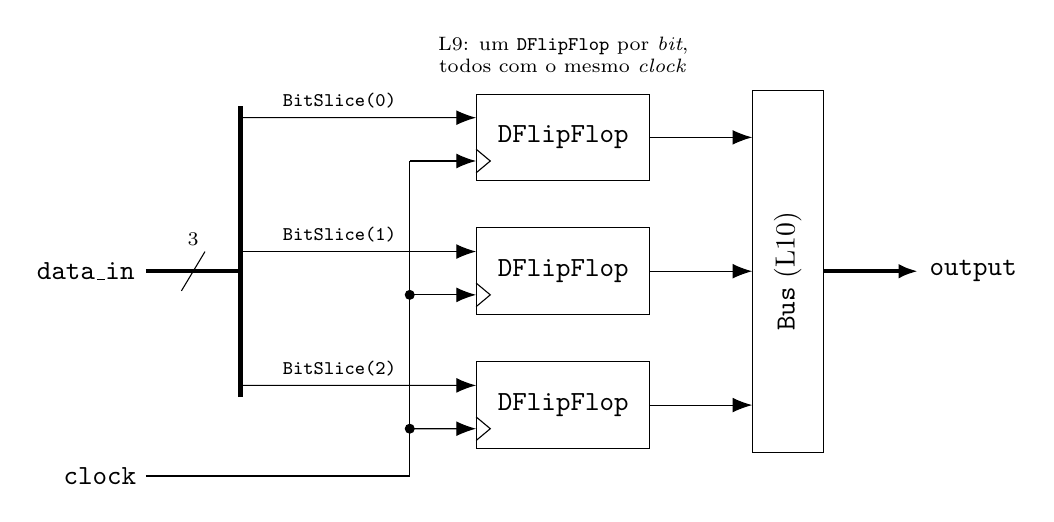
\begin{tikzpicture}[>={Latex[length=2.5mm]}]
    \foreach \i/\y in {0/1.7, 1/0, 2/-1.7} {
        \node[draw, minimum width=2.2cm, minimum height=1.1cm] (ff\i) at (4.7,\y) {\texttt{DFlipFlop}};
        \draw[->] (0.6,\y+0.25) -- ($(ff\i.west)+(0,0.25)$) node[pos=0.42, above, font=\scriptsize]{\texttt{BitSlice(\i)}};
        \draw[->] (2.75,\y-0.3) -- ($(ff\i.west)+(0,-0.3)$);
        \draw ($(ff\i.west)+(0,-0.45)$) -- ++(0.18,0.15) -- ++(-0.18,0.15);
        \draw[->] (ff\i.east) -- (7.1,\y);
    }
    \draw[line width=1.6pt] (0.6,-1.6) -- (0.6,2.1);
    \draw[line width=1.6pt] (-0.6,0) node[left]{\texttt{data\_in}} -- (0.6,0);
    \draw (-0.15,-0.25) -- (0.15,0.25);
    \node[above, font=\scriptsize] at (0,0.2) {3};
    \draw (-0.6,-2.6) node[left]{\texttt{clock}} -- (2.75,-2.6) -- (2.75,1.4);
    \foreach \y in {-0.3, -2.0} { \node[circ] at (2.75,\y) {}; }
    \node[draw, minimum width=0.9cm, minimum height=4.6cm, align=center] (bus) at (7.55,0) {\rotatebox{90}{\texttt{Bus} (L10)}};
    \draw[->, line width=1.6pt] (bus.east) -- ++(1.2,0) node[right]{\texttt{output}};
    \node[font=\scriptsize, align=center] at (4.7,2.75) {L9: um \texttt{DFlipFlop} por \textit{bit},\\todos com o mesmo \textit{clock}};
\end{tikzpicture}
\begin{center}
\footnotesize Fonte: elaborada pelo autor (2026).
\end{center}
\end{figure}

O construtor do \texttt{DFlipFlopRegister} tem exatamente a mesma assinatura do \texttt{BehavioralRegister} (\texttt{clock}, \texttt{data\_in}, \texttt{feedback\_target}), o que permite trocar um pelo outro em qualquer circuito de exemplo sem alterar mais nada além do nome da classe instanciada, como no contador da Seção~\ref{sec:composicao}. Isso torna direta a comparação entre a abstração e sua contraparte real, validada na Seção~\ref{sec:contador-portas-real}.

\section{Composição de Circuitos}
\label{sec:composicao}

Os componentes descritos nas seções anteriores foram combinados para construir e validar os circuitos de exemplo a seguir. Diferentemente dos algoritmos apresentados até aqui, que reproduzem trechos da biblioteca em si, os exemplos a seguir mostram código de uso: código escrito pelo estudante para compor um circuito a partir dos componentes já prontos.

\subsection{Meio-Somador}

Um meio-somador é obtido diretamente pela composição de uma porta \texttt{Xor} (soma) e uma porta \texttt{And} (\textit{carry}) sobre as mesmas duas entradas de um \textit{bit}, como mostra o Exemplo~\ref{ex:meio-somador}.

\begin{exemplo}[H]
\caption{Meio-somador composto a partir de Xor e And.}
\label{ex:meio-somador}
\begin{minted}{python}
bx, by = BitArray([x]), BitArray([y])
soma = Xor(bx, by)
carry = And(bx, by)
\end{minted}
\begin{center}
\footnotesize Fonte: elaborado pelo autor (2026).
\end{center}
\end{exemplo}

\subsection{Somador Completo}

O mesmo meio-somador, estendido com um terceiro sinal de \textit{carry} de entrada, é o próprio \texttt{FullAdder} apresentado no Algoritmo~\ref{alg:fulladder}: basta instanciá-lo com três sinais de 1 \textit{bit} (\texttt{a}, \texttt{b}, \texttt{carry\_in}) e ler \texttt{.sum} e \texttt{.carry\_out}.

\subsection{Contador Binário Realimentado com \texttt{BehavioralAdder}}

Esta é a versão mais simples do contador, usada quando o foco é demonstrar o registrador e a realimentação. No Exemplo~\ref{ex:contador-behavioral}, um \texttt{BehavioralAdder} soma continuamente uma constante (\texttt{001}) ao valor atual do próprio contador, e um \texttt{BehavioralRegister} captura esse novo valor a cada pulso de \textit{clock}, devolvendo-o ao mesmo sinal que alimenta o somador.

\begin{exemplo}[H]
\caption{Contador binário de N \textit{bits} com BehavioralAdder.}
\label{ex:contador-behavioral}
\begin{minted}{python}
increment = BitArray([False, False, True])       # constante 001
counter_value = BitArray([False, False, False])  # valor atual do contador

adder = BehavioralAdder(increment, counter_value)      # soma = counter_value + 001
clock = BitArray(False)
counter = BehavioralRegister(clock, adder, feedback_target=counter_value)  # realimenta
\end{minted}
\begin{center}
\footnotesize Fonte: elaborado pelo autor (2026).
\end{center}
\end{exemplo}

A Figura~\ref{fig:propagacao} ilustra a cadeia de propagação desse circuito: a cada pulso de \textit{clock}, o \texttt{BehavioralRegister} lê a saída atual do \texttt{BehavioralAdder}, atualiza \texttt{counter\_value}, e essa atualização dispara automaticamente um novo cálculo do \texttt{BehavioralAdder}, deixando o circuito pronto para o próximo pulso.

\subsection{Contador Binário Realimentado com Portas Lógicas}

Substituindo o \texttt{BehavioralAdder} pelo \texttt{RippleCarryAdder}, como no Exemplo~\ref{ex:contador-portas}, o mesmo contador passa a ter a soma montada inteiramente com portas lógicas, e o \textit{overflow} do 8º pulso deixa de depender de \texttt{pad\_binary\_array}, aparecendo diretamente no \texttt{carry\_out} do somador.

\begin{exemplo}[H]
\caption{Contador binário de N \textit{bits} com somador de portas lógicas.}
\label{ex:contador-portas}
\begin{minted}{python}
increment = BitArray([False, False, True])
counter_value = BitArray([False, False, False])
adder = RippleCarryAdder(counter_value, increment)

clock = BitArray(False)
counter = BehavioralRegister(clock, adder.sum, feedback_target=counter_value)
\end{minted}
\begin{center}
\footnotesize Fonte: elaborado pelo autor (2026).
\end{center}
\end{exemplo}

\subsection{Contador Binário Realimentado com Registrador Real}
\label{sec:contador-registrador-real}

Trocando também o \texttt{BehavioralRegister} pelo \texttt{DFlipFlopRegister} (Seção~\ref{sec:dflipflop-register}), como no Exemplo~\ref{ex:contador-real}, o mesmo contador passa a ser montado do início ao fim só com portas lógicas, sem nenhuma abstração de borda de \textit{clock} em Python: tanto a soma quanto o armazenamento do valor entre pulsos são reproduzidos a partir de \textit{latches} e portas. O sinal de \texttt{clock} precisa ser um \texttt{BitArray} de 1 \textit{bit} em lista (\texttt{[False]}, e não \texttt{False}), pois agora ele alimenta diretamente portas lógicas (o \texttt{Not} de cada \texttt{DFlipFlop}), que operam sobre listas de \textit{bits}; o \texttt{BehavioralRegister}, por sua vez, aceita as duas formas.

\begin{exemplo}[H]
\caption{Contador binário de N \textit{bits} com registrador real (DFlipFlopRegister).}
\label{ex:contador-real}
\begin{minted}{python}
increment = BitArray([False, False, True])
counter_value = BitArray([False, False, False])
adder = RippleCarryAdder(counter_value, increment)

clock = BitArray([False])
counter = DFlipFlopRegister(clock, adder.sum, feedback_target=counter_value)
\end{minted}
\begin{center}
\footnotesize Fonte: elaborado pelo autor (2026).
\end{center}
\end{exemplo}

Esse contador é validado e comparado ao seu equivalente com \texttt{BehavioralRegister} na Seção~\ref{sec:contador-portas-real}.

\subsection{\textit{Flip-Flop Toggle}}

O mesmo padrão de realimentação, substituindo o somador por uma porta \texttt{Xor} com uma constante \texttt{1}, produz um \textit{flip-flop} do tipo \textit{toggle}, cuja saída se inverte a cada pulso de \textit{clock}, como mostra o Exemplo~\ref{ex:toggle}.

\begin{exemplo}[H]
\caption{\textit{Flip-flop} \textit{toggle}.}
\label{ex:toggle}
\begin{minted}{python}
one = BitArray([True])
clock = BitArray(False)
signal = BitArray([False])

toggle_logic = Xor(signal, one)
flip_flop = BehavioralRegister(clock, toggle_logic, feedback_target=signal)
\end{minted}
\begin{center}
\footnotesize Fonte: elaborado pelo autor (2026).
\end{center}
\end{exemplo}

Esses circuitos, junto com o comportamento dos três contadores em oito ou nove pulsos de \textit{clock} (incluindo o \textit{overflow}), são validados e discutidos no Capítulo~\ref{cap:resultados}.

\section{Tecnologias Utilizadas}

O simulador foi implementado em Python 3, utilizando exclusivamente recursos da biblioteca padrão da linguagem, sem nenhuma dependência externa. Essa escolha reforça o objetivo do trabalho: o estudante pode executar e modificar o simulador com qualquer instalação padrão de Python, sem a necessidade de instalar ou configurar ferramentas adicionais. Cada módulo e cada classe da biblioteca possui uma \textit{docstring} descrevendo seu papel, de modo que a documentação de uso básico esteja disponível diretamente no código (por exemplo, via \texttt{help(BitArray)}), complementando a descrição arquitetural apresentada neste capítulo. Os testes automatizados descritos na Seção~\ref{sec:testes} também usam apenas o módulo \texttt{unittest} da biblioteca padrão.

\section{A \textit{Engine} de Propagação}
\label{sec:motor-interno}

Reunindo o que as seções anteriores apresentaram separadamente, a \textit{engine} deste simulador não é um módulo à parte: é o próprio contrato descrito na Seção~\ref{sec:visao-arquitetura} (\texttt{output}, \texttt{add\_listener}, \texttt{trigger\_change}), repetido em cada classe. Não existe um laço central de simulação, um agendador, nem uma noção de tempo ou de ``ciclo de \textit{clock} global'': a propagação inteira acontece dentro da pilha de chamadas do próprio Python, disparada pela primeira atribuição feita pelo código cliente (tipicamente, alternar um \texttt{BitArray} de \textit{clock}).

A Figura~\ref{fig:diagrama-sequencia} traduz essa ideia para o caso concreto do \textit{flip-flop} \textit{toggle} (Seção~\ref{sec:composicao}), reproduzindo, como diagrama de sequência UML, o mesmo log real de propagação apresentado na Seção~\ref{sec:log-propagacao}: uma única atribuição externa (\texttt{clock.output = True}) desencadeia uma cadeia de três chamadas de \texttt{trigger\_change} em sequência, cada uma completada antes que a próxima comece, até o circuito se estabilizar.

\begin{figure}[H]
\centering
\caption{Diagrama de sequência de um pulso de \textit{clock} no \textit{flip-flop} \textit{toggle}.}
\label{fig:diagrama-sequencia}
\resizebox{\textwidth}{!}{%
\begin{sequencediagram}
\newinst{cliente}{:cliente}
\newinst[2]{clock}{clock:BitArray}
\newinst[2]{ff}{flip\_flop:BehavioralRegister}
\newinst[2]{signal}{signal:BitArray}
\newinst[2]{toggle}{toggle\_logic:Xor}

\mess{cliente}{output = True}{clock}
\mess{clock}{clock subiu}{ff}
\mess{ff}{captura e realimenta}{signal}
\mess{signal}{recalcula}{toggle}
\end{sequencediagram}%
}
\begin{center}
\footnotesize Fonte: elaborada pelo autor (2026), com base no log de execução real da Seção~\ref{sec:log-propagacao}.
\end{center}
\end{figure}

Três decisões de projeto, tomadas em conjunto, definem o comportamento observável dessa \textit{engine}:

\begin{itemize}
    \item \textbf{Notificação em cadeia síncrona}: quando \texttt{output} de um componente muda, ele chama, um a um, os \textit{listeners} registrados (Linha 16 do Algoritmo~\ref{alg:bitarray}, \texttt{for listener in self.\_listeners}), e cada chamada de \textit{listener} pode, por sua vez, disparar uma nova cadeia de notificações antes de retornar. Isso significa que a propagação de uma única mudança de sinal é resolvida inteiramente antes que o código cliente recupere o controle: não há filas de eventos nem execução assíncrona;
    \item \textbf{Ordem de notificação}: os \textit{listeners} de um mesmo componente são percorridos na ordem em que foram registrados. Para os circuitos combinacionais e para os circuitos sequenciais construídos sobre o \texttt{BehavioralRegister}, a ordem de notificação não altera o resultado final, pois cada componente recalcula seu próprio estado de forma independente a partir das entradas atuais, e não da ordem de chegada das notificações. Ela deixa de ser um detalhe inofensivo, porém, quando dois componentes que deveriam se ``revezar'' (como o \textit{latch} mestre e o \textit{latch} escravo do \texttt{DFlipFlop}, Seção~\ref{sec:latches}) dependem do mesmo sinal de \texttt{clock}: nesse caso, a ordem determina qual dos dois reage primeiro a uma mudança, e é por isso que \texttt{not\_clock} é registrado como \textit{listener} de \texttt{clock} antes das portas do \textit{latch} escravo (que só existem depois que o \textit{latch} mestre, e portanto \texttt{not\_clock}, já foi construído): como a notificação segue a ordem de registro, o mestre sempre fecha antes de o escravo abrir. Essa validação é apresentada na Seção~\ref{sec:contador-portas-real};
    \item \textbf{Filtragem por igualdade}: cada componente só recalcula seu \texttt{\_output} e notifica seus \textit{listeners} quando o novo valor calculado difere do anterior (Linhas 13 e 14 do Algoritmo~\ref{alg:bitarray}). Sem esse filtro, um laço de realimentação combinacional genuíno (como o do \texttt{SRLatch}, Seção~\ref{sec:latches}) reentraria indefinidamente na mesma cadeia de chamadas.
\end{itemize}

Essas três regras bastam para explicar tanto os circuitos que funcionam quanto os que podem não estabilizar: um circuito acíclico (qualquer composição de portas sem realimentação) sempre termina de propagar em um número finito de passos, pois cada componente é notificado uma vez por mudança de entrada; um circuito com realimentação que passa por um \texttt{BehavioralRegister} também termina, porque o \texttt{BehavioralRegister} só propaga adiante no instante controlado da borda de \textit{clock}, e não a cada mudança intermediária de \texttt{data\_in}; um circuito com realimentação através de \textit{latches} (o \texttt{SRLatch} ou o \texttt{DFlipFlop} mestre-escravo, Seção~\ref{sec:latches}) também termina, mas depende, além do filtro por igualdade, de que a ordem de notificação respeite a ordem em que os componentes foram construídos (mestre antes de escravo), para que a alternância de transparência entre os dois \textit{latches} funcione como um mecanismo de corte equivalente ao do \texttt{BehavioralRegister}. Se essa ordem não fosse respeitada, o circuito degeneraria em um laço puramente combinacional com uma única inversão, sem ponto fixo algum, independentemente do filtro por igualdade.

\chapter{Resultados e Discussão}
\label{cap:resultados}

Este capítulo apresenta os resultados obtidos com a execução dos circuitos de exemplo descritos no Capítulo~\ref{cap:proposta}, comparando a saída produzida pelo simulador com o comportamento teoricamente esperado. Em seguida, descrevem-se os testes automatizados que verificam esses resultados e os recursos de observação e depuração que o simulador oferece, comparados aos de outras ferramentas, e discutem-se as limitações da abordagem.

\section{Validação dos Circuitos Implementados}
\label{sec:validacao}

Esta seção percorre, em ordem crescente de complexidade, a validação de cada circuito descrito no Capítulo~\ref{cap:proposta}: da propagação reativa em uma única porta lógica até os três contadores binários e o \textit{flip-flop} \textit{toggle}, incluindo a validação do registrador construído com \textit{latches}.

\subsection{Porta NOT Reativa}

O primeiro teste verifica se uma porta lógica recalcula sua saída automaticamente quando sua entrada muda, sem que nenhum código externo solicite esse recálculo. Partindo de \texttt{a = BitArray([False, True, False])} e \texttt{not\_a = Not(a)}, obteve-se o resultado apresentado na Tabela~\ref{tab:not}.

\begin{table}[H]
\centering
\caption{Propagação reativa através de uma porta NOT.}
\label{tab:not}
\begin{tabular}{l|l}
\hline
\textbf{Evento} & \textbf{not\_a.output} \\
\hline
Estado inicial (\texttt{a = [F, T, F]}) & \texttt{[T, F, T]} \\
Após \texttt{a.output = [T, T, T]} & \texttt{[F, F, F]} \\
\hline
\end{tabular}
\begin{center}
\footnotesize Fonte: elaborada pelo autor (2026), com base na execução do simulador.
\end{center}
\end{table}

O resultado confirma que a alteração de \texttt{a.output} propagou-se automaticamente para \texttt{not\_a}, sem qualquer chamada explícita a um método de recálculo, validando o mecanismo de notificação descrito na Seção~\ref{sec:sinais}.

\subsection{Meio-Somador e Somador Completo}

O meio-somador (\texttt{Xor} para soma, \texttt{And} para \textit{carry}) foi testado com as quatro combinações possíveis de entrada de 1 \textit{bit}, reproduzindo exatamente a tabela-verdade esperada. O mesmo teste foi repetido para o \texttt{FullAdder} (Seção~\ref{sec:somador-portas}), incluindo agora um \textit{carry} de entrada. Os dois resultados são apresentados na Tabela~\ref{tab:somadores}.

\begin{table}[H]
\centering
\caption{Saída do meio-somador e do somador completo comparadas à tabela-verdade esperada.}
\label{tab:somadores}
\begin{tabular}{ccc|cc}
\hline
$A$ & $B$ & $C_{in}$ & Soma & \textit{Carry-out} \\
\hline
\multicolumn{5}{l}{\textit{Meio-somador (sem carry de entrada)}} \\
\hline
0 & 0 & -- & 0 & 0 \\
0 & 1 & -- & 1 & 0 \\
1 & 0 & -- & 1 & 0 \\
1 & 1 & -- & 0 & 1 \\
\hline
\multicolumn{5}{l}{\textit{Somador completo (8 combinações de $A$, $B$ e $C_{in}$)}} \\
\hline
0 & 0 & 0 & 0 & 0 \\
0 & 0 & 1 & 1 & 0 \\
0 & 1 & 0 & 1 & 0 \\
0 & 1 & 1 & 0 & 1 \\
1 & 0 & 0 & 1 & 0 \\
1 & 0 & 1 & 0 & 1 \\
1 & 1 & 0 & 0 & 1 \\
1 & 1 & 1 & 1 & 1 \\
\hline
\end{tabular}
\begin{center}
\footnotesize Fonte: elaborada pelo autor (2026), com base na execução do simulador.
\end{center}
\end{table}

Todos os valores obtidos corresponderam exatamente ao esperado pela álgebra booleana (Seção~\ref{sec:algebra-booleana}), tanto para o meio-somador (linhas superiores, sem \textit{carry} de entrada) quanto para o somador completo.


\subsection{Registrador Simples}

Um \texttt{BehavioralRegister} sem realimentação foi usado para validar a detecção de borda de subida isoladamente: antes de qualquer pulso de \textit{clock}, \texttt{register.output} permanece \texttt{None}; após \texttt{clock.output = True}, o valor de \texttt{data\_in.output} no instante da borda é capturado e mantido, mesmo que \texttt{data\_in.output} mude posteriormente sem um novo pulso de \textit{clock}, e mesmo quando o \textit{clock} volta a falso (borda de descida). O mesmo comportamento foi verificado com o \textit{clock} representado tanto como booleano (\texttt{BitArray(False)}) quanto como lista de um \textit{bit} (\texttt{BitArray([False])}). Esse comportamento confirma que o \texttt{BehavioralRegister} reage apenas à borda de subida do sinal de \textit{clock}, e não a mudanças na entrada de dados.

\subsection{Contador Binário e \textit{Flip-Flop Toggle}}
\label{sec:log-propagacao}

Os dois circuitos com laço de realimentação foram validados pulsando o \textit{clock} repetidamente e comparando a sequência de saídas com a esperada para, respectivamente, um contador binário crescente (usando \texttt{BehavioralAdder}) e um \textit{flip-flop} que inverte de estado a cada pulso. As duas sequências obtidas são apresentadas na Tabela~\ref{tab:contador-toggle}.

\begin{table}[H]
\centering
\caption{Saída do contador de 3 \textit{bits} e do \textit{flip-flop} \textit{toggle} ao longo de sucessivos pulsos de \textit{clock}.}
\label{tab:contador-toggle}
\begin{tabular}{c|l|l}
\hline
\textbf{Pulso} & \textbf{Contador (3 bits)} & \textbf{\textit{Flip-flop} \textit{toggle}} \\
\hline
1 & 001 & 1 \\
2 & 010 & 0 \\
3 & 011 & 1 \\
4 & 100 & 0 \\
5 & 101 & 1 \\
6 & 110 & 0 \\
7 & 111 & --- \\
\hline
\end{tabular}
\begin{center}
\footnotesize Fonte: elaborada pelo autor (2026), com base na execução do simulador.
\end{center}
\end{table}

Ambas as sequências corresponderam exatamente ao esperado: o contador incrementa uma unidade a cada pulso, e o \textit{flip-flop} \textit{toggle} alterna seu estado, confirmando que o \texttt{BehavioralRegister} realimentado é capaz de sustentar um circuito com estado persistente ao longo de múltiplos ciclos de \textit{clock}.

Para tornar visível a ordem real de propagação dentro de um único pulso, um \textit{listener} de registro (\textit{log}) foi anexado a cada componente do circuito do \textit{flip-flop} \textit{toggle}. O Quadro~\ref{qua:log-toggle} mostra a saída obtida para um único pulso de \textit{clock}, evidenciando como o sinal se propaga em cadeia até se estabilizar.

\begin{quadro}[H]
\centering
\caption{Log de propagação de um pulso de \textit{clock} no \textit{flip-flop} \textit{toggle}.}
\label{qua:log-toggle}
\begin{minipage}{0.6\textwidth}
\begin{verbatim}
estado antes do pulso: signal = [False]
pulso de clock (False -> True):
  toggle_logic: [True] -> [False]
  signal:       [False] -> [True]
  flip_flop:    [False] -> [True]
  clock:        False -> True
estado apos o pulso: signal = [True]
\end{verbatim}
\end{minipage}
\begin{center}
\footnotesize Fonte: elaborado pelo autor (2026), com base na execução do simulador.
\end{center}
\end{quadro}

A ordem desse log só faz sentido à luz de como cada linha é impressa: o \textit{listener} de log foi registrado em cada sinal \textbf{depois} do \textit{listener} funcional que já existia desde a Seção~\ref{sec:composicao} (o próprio \texttt{BehavioralRegister}, no caso de \texttt{clock} e \texttt{flip\_flop}; o próprio \texttt{Xor}, no caso de \texttt{signal}), e a \textit{engine} notifica \textit{listeners} na ordem em que foram registrados (Seção~\ref{sec:motor-interno}). Assim, a atribuição \texttt{clock.output = True} primeiro dispara o \texttt{BehavioralRegister} (\texttt{flip\_flop}), que lê o valor já estabilizado de \texttt{toggle\_logic} (\texttt{True}) e o propaga para \texttt{signal}, que por sua vez dispara o recálculo de \texttt{toggle\_logic} (\texttt{False}) antes de qualquer linha ser impressa; só então, à medida que cada chamada de \texttt{trigger\_change} retorna, os quatro \textit{listeners} de log dessa cadeia disparam em ordem inversa à da causa: primeiro o de \texttt{toggle\_logic} (o mais interno, que recalculou por último), depois \texttt{signal}, depois \texttt{flip\_flop}, e por fim o de \texttt{clock} (o mais externo, que só é notificado quando a pilha de chamadas termina de desenrolar). Nenhum desses quatro componentes é notificado mais de uma vez, o que confirma que o circuito se estabiliza em uma única passada de propagação para esse caso.

\subsection{Contador Binário Montado Só com Portas Lógicas}
\label{sec:contador-portas}

O mesmo contador foi refeito trocando o \texttt{BehavioralAdder} pelo \texttt{RippleCarryAdder} (Seção~\ref{sec:somador-portas}), permitindo observar também o sinal \texttt{carry\_out} a cada pulso, como mostra a Tabela~\ref{tab:contador-portas}.

\begin{table}[H]
\centering
\caption{Contador de 3 \textit{bits} montado com RippleCarryAdder, com carry\_out.}
\label{tab:contador-portas}
\begin{tabular}{c|l|l}
\hline
\textbf{Pulso} & \textbf{Contador (3 bits)} & \textbf{carry\_out} \\
\hline
1 & 001 & 0 \\
2 & 010 & 0 \\
3 & 011 & 0 \\
4 & 100 & 0 \\
5 & 101 & 0 \\
6 & 110 & 0 \\
7 & 111 & 1 \\
8 & 000 & 0 \\
9 & 001 & 0 \\
\hline
\end{tabular}
\begin{center}
\footnotesize Fonte: elaborada pelo autor (2026), com base na execução do simulador.
\end{center}
\end{table}

O resultado reproduziu exatamente a sequência do contador com \texttt{BehavioralAdder}, com uma diferença importante: no pulso 7, assim que o valor \texttt{111} é realimentado para a entrada do somador, \texttt{carry\_out} sobe para \texttt{1}, sinalizando que a próxima soma (\texttt{111 + 001}) excede 3 \textit{bits}. No pulso 8, o \texttt{BehavioralRegister} captura a soma já ``estourada'' (\texttt{000}), e \texttt{carry\_out} volta a \texttt{0} porque a nova entrada do somador (\texttt{000}) não gera mais \textit{overflow}. Esse resultado confirma, na prática, o que foi projetado na Seção~\ref{sec:somador-portas}: o \textit{overflow} de um somador montado com portas lógicas aparece naturalmente em um sinal de \textit{carry} separado, sem exigir nenhum tratamento especial em código.

\subsection{Registrador Real com \textit{Latches}}
\label{sec:contador-portas-real}

O \textit{latch} SR (Seção~\ref{sec:latches}) foi validado com a sequência clássica de \textit{set}, \textit{hold} e \textit{reset}, reproduzindo exatamente o comportamento esperado, como mostra a Tabela~\ref{tab:sr-latch}.

\begin{table}[H]
\centering
\caption{Validação do \textit{latch} SR (NOR cruzado).}
\label{tab:sr-latch}
\begin{tabular}{cc|l}
\hline
$S$ & $R$ & $Q$ \\
\hline
1 & 0 & \texttt{[True]} (\textit{set}) \\
0 & 0 & \texttt{[True]} (\textit{hold}, mantém o valor anterior) \\
0 & 1 & \texttt{[False]} (\textit{reset}) \\
0 & 0 & \texttt{[False]} (\textit{hold}, mantém o valor anterior) \\
\hline
\end{tabular}
\begin{center}
\footnotesize Fonte: elaborada pelo autor (2026), com base na execução do simulador.
\end{center}
\end{table}

O \texttt{DFlipFlop} (Seção~\ref{sec:latches}) foi então validado com um sinal $D$ independente, alternando o \textit{clock} e o próprio $D$ em momentos distintos para confirmar a sensibilidade exclusiva à borda de subida. A saída produzida pelo programa \texttt{experiments.py} é apresentada no Quadro~\ref{qua:dff}.

\begin{quadro}[H]
\centering
\caption{Validação do \texttt{DFlipFlop} isolado.}
\label{qua:dff}
\begin{minipage}{0.9\textwidth}
\begin{verbatim}
D=1, clock sobe -> Q=[True] (capturou D)
D muda p/ 0 com clock ainda em 1 -> Q=[True] (nao muda)
clock desce (1->0) -> Q=[True] (flip-flop so muda na borda de subida)
clock sobe de novo com D=0 -> Q=[False] (capturou o novo D)
\end{verbatim}
\end{minipage}
\begin{center}
\footnotesize Fonte: elaborado pelo autor (2026), com base na execução do simulador.
\end{center}
\end{quadro}

O resultado confirma que o \texttt{DFlipFlop} reproduz, a partir de portas lógicas reais, o mesmo comportamento observável do \texttt{BehavioralRegister}: a saída só se atualiza no instante da borda de subida do \textit{clock}, permanecendo estável mesmo que $D$ mude enquanto o \textit{clock} está em nível alto ou baixo.

O \textit{flip-flop} \textit{toggle} da Seção~\ref{sec:composicao} foi então reproduzido substituindo o \texttt{BehavioralRegister} pelo \texttt{DFlipFlop} (isto é, realimentando a própria saída, invertida, de volta para a entrada $D$). Diferentemente do \texttt{BehavioralRegister}, que quebra qualquer ciclo de realimentação lendo \texttt{data\_in} apenas no instante exato da borda de \textit{clock}, o \texttt{DFlipFlop} depende inteiramente da separação de transparência entre o \textit{latch} mestre e o \textit{latch} escravo (Seção~\ref{sec:latches}) para que essa realimentação não degenere em um laço puramente combinacional: a ordem de notificação do simulador (Seção~\ref{sec:motor-interno}) garante que \texttt{not\_clock} feche o \textit{latch} mestre antes de as portas do \textit{latch} escravo serem notificadas, preservando essa separação a cada pulso de \textit{clock}. O resultado é apresentado na Tabela~\ref{tab:toggle-dff}.

\begin{table}[H]
\centering
\caption{Saída do \textit{flip-flop} \textit{toggle} montado com DFlipFlop.}
\label{tab:toggle-dff}
\begin{tabular}{c|l}
\hline
\textbf{Pulso} & \textbf{Saída} \\
\hline
Estado inicial & 1 \\
1 & 0 \\
2 & 1 \\
3 & 0 \\
4 & 1 \\
5 & 0 \\
6 & 1 \\
\hline
\end{tabular}
\begin{center}
\footnotesize Fonte: elaborada pelo autor (2026), com base na execução do simulador.
\end{center}
\end{table}

A sequência alterna estritamente a cada pulso, com o mesmo padrão observado para o \textit{flip-flop} \textit{toggle} construído sobre o \texttt{BehavioralRegister} (Seção~\ref{sec:log-propagacao}), a menos de uma defasagem de fase: o estado inicial começa em 1 em vez de 0. Em um circuito físico, o valor de $Q$ antes do primeiro pulso de \textit{clock} seria indeterminado; no simulador, ele é sempre o mesmo, mas arbitrário: decorre do valor inicial atribuído ao \texttt{BitArray} de proxy usado para fechar o laço do \texttt{SRLatch} (\texttt{[False]}, Linha 7 do Algoritmo~\ref{alg:srlatch}), que faz com que $Q = \overline{R}$ na construção e, portanto, $Q = 1$ enquanto o \textit{latch} não está habilitado. Trata-se de um artefato da inicialização, e não de um defeito na propagação.

Para validar esse comportamento em uma escala maior do que um único \textit{flip-flop}, o contador de 3 \textit{bits} montado com \texttt{RippleCarryAdder} (Seção~\ref{sec:contador-portas}) foi reconstruído trocando também o \texttt{BehavioralRegister} pelo \texttt{DFlipFlopRegister} (Seção~\ref{sec:dflipflop-register}), um registrador de N \textit{bits} montado inteiramente com portas lógicas. A Tabela~\ref{tab:comparacao-registradores} compara o resultado, lado a lado, com o contador de referência (que usa o \texttt{BehavioralRegister}).

\begin{table}[H]
\centering
\caption{Contador de 3 \textit{bits} com BehavioralRegister comparado ao mesmo contador com DFlipFlopRegister.}
\label{tab:comparacao-registradores}
\begin{tabular}{c|l|l}
\hline
\textbf{Pulso} & \textbf{BehavioralRegister} & \textbf{DFlipFlopRegister} \\
\hline
Estado inicial & \texttt{None} & 111 \\
1 & 001 & 000 \\
2 & 010 & 001 \\
3 & 011 & 010 \\
4 & 100 & 011 \\
5 & 101 & 100 \\
6 & 110 & 101 \\
7 & 111 (carry\_out=1) & 110 \\
8 & 000 & 111 (carry\_out=1) \\
9 & 001 & 000 \\
\hline
\end{tabular}
\begin{center}
\footnotesize Fonte: elaborada pelo autor (2026), com base na execução do simulador.
\end{center}
\end{table}

As duas sequências são idênticas, inclusive no pulso em que o \textit{overflow} ocorre, a menos da mesma defasagem de uma posição já explicada para o \textit{flip-flop} \textit{toggle}: o \texttt{DFlipFlopRegister} começa em \texttt{111} porque cada um dos três \texttt{DFlipFlop} que o compõem parte do mesmo valor inicial arbitrário ($Q = 1$) antes do primeiro pulso de \textit{clock}. Esse resultado estende a validação de um único \textit{bit} realimentado para um registrador completo de N \textit{bits}, sem que nenhuma das duas classes (\texttt{BehavioralRegister} e \texttt{DFlipFlopRegister}) precisasse de qualquer ajuste específico para lidar com múltiplos \textit{bits}: o \texttt{DFlipFlopRegister} reaproveita, sem alterações, a mesma técnica de composição por \texttt{BitSlice} e \texttt{Bus} já usada pelo \texttt{RippleCarryAdder} (Seção~\ref{sec:somador-portas}). Vale notar o escopo dessa validação: ela comprova que este caso específico, exaustivamente testado, estabiliza corretamente, mas não que toda topologia de realimentação combinacional através de \textit{latches} estabiliza sob a mesma convenção de ordenação, ressalva retomada na Seção~\ref{sec:limitacoes}.

\section{Testes Automatizados}
\label{sec:testes}

Os resultados apresentados na seção anterior foram inicialmente obtidos executando o programa \texttt{experiments.py} (Apêndice~\ref{ap:testes-exemplos}) e comparando visualmente sua saída com o comportamento esperado. Para que essa validação seja reproduzível e não dependa de inspeção manual, cada um desses resultados foi transformado em um caso de teste automatizado no arquivo \texttt{tests/test\_circuitos.py} (Apêndice~\ref{ap:testes-exemplos}), escrito com o módulo \texttt{unittest} da biblioteca padrão de Python. Os testes verificam, por meio de asserções, a porta NOT reativa, o meio-somador, o somador completo nas oito combinações de entrada, o \texttt{RippleCarryAdder} de 3 \textit{bits} em todas as 64 combinações de operandos (incluindo o \texttt{carry\_out}), a captura do \texttt{BehavioralRegister} apenas na borda de subida, os três contadores ao longo de nove pulsos de \textit{clock}, o \textit{latch} SR, o \texttt{DFlipFlop} isolado e os dois \textit{flip-flops} \textit{toggle}.

Um dos testes cobre especificamente o defeito de detecção de borda do \texttt{BehavioralRegister} descrito na Seção~\ref{sec:register}: com o \textit{clock} representado como lista (\texttt{BitArray([False])}), ele verifica que o valor capturado não muda na borda de descida. Esse teste falhava com a versão anterior do componente e passa com a versão atual. Os treze testes são executados com o comando \texttt{python -m unittest discover -s tests -t .} e, na versão final do simulador, todos passam.

\section{Recursos de Observação e Depuração}
\label{sec:observacao}

Como cada componente do simulador é um objeto Python comum, e a propagação acontece por chamadas de função entre esses objetos (Seção~\ref{sec:motor-interno}), o estudante pode observar e interrogar o circuito usando a mesma linguagem com que o construiu, sem nenhuma ferramenta adicional. Dois desses recursos já foram usados neste capítulo: a impressão do estado a cada ciclo de \textit{clock} (Tabelas~\ref{tab:contador-toggle} a \ref{tab:comparacao-registradores}) e o registro da ordem de propagação dentro de um único pulso (Quadro~\ref{qua:log-toggle}). Esta seção apresenta outros cinco, todos reunidos no programa \texttt{recursos\_observacao.py} (Apêndice~\ref{ap:testes-exemplos}) e executados para produzir as saídas reproduzidas a seguir, e compara esses recursos aos oferecidos pelas ferramentas discutidas no Capítulo~\ref{cap:trabalhos}.

\subsection{Estados Transitórios (\textit{Glitches})}

Em um somador estrutural, o resultado não aparece de uma só vez: cada estágio só pode calcular sua soma depois de receber o \textit{carry} do estágio anterior, e a saída passa por valores intermediários até se estabilizar. No simulador, basta registrar um \textit{listener} na saída do somador para observar esses valores. O Exemplo~\ref{ex:transitorios} monta, sobre as mesmas entradas, um \texttt{RippleCarryAdder} e um \texttt{BehavioralAdder} de 4 \textit{bits}, e altera a entrada \texttt{b} de forma que o \textit{carry} precise atravessar três estágios ($0111 + 0001$).

\begin{exemplo}[H]
\caption{Observação dos estados transitórios de um somador.}
\label{ex:transitorios}
\begin{minted}{python}
a = BitArray([False, True, True, True])      # 0111
b = BitArray([False, False, False, False])   # 0000
estrutural = RippleCarryAdder(a, b).sum
comportamental = BehavioralAdder(a, b)
estrutural.add_listener(lambda old, new: print("estrutural:    ", bits(new)))
comportamental.add_listener(lambda old, new: print("comportamental:", bits(new)))
b.output = [False, False, False, True]       # 0111 + 0001 = 1000
\end{minted}
\begin{center}
\footnotesize Fonte: elaborado pelo autor (2026).
\end{center}
\end{exemplo}

O Quadro~\ref{qua:transitorios} mostra que a saída do somador estrutural passou por três valores intermediários antes de chegar a \texttt{1000}, enquanto o somador comportamental, que calcula a soma de uma vez em Python, passou diretamente ao resultado final.

\begin{quadro}[H]
\centering
\caption{Saídas observadas durante a propagação do Exemplo~\ref{ex:transitorios}.}
\label{qua:transitorios}
\begin{minipage}{0.5\textwidth}
\begin{verbatim}
estrutural:     0110
estrutural:     1110
estrutural:     1010
estrutural:     1000
comportamental: 1000
\end{verbatim}
\end{minipage}
\begin{center}
\footnotesize Fonte: elaborado pelo autor (2026), com base na execução do simulador.
\end{center}
\end{quadro}

Esse resultado torna visível, de forma concreta, a diferença entre as duas descrições e a natureza sequencial da propagação do \textit{carry} em um \textit{ripple-carry adder}. É preciso, porém, interpretá-lo com cuidado: como o simulador não modela atraso de propagação (Seção~\ref{sec:limitacoes}), a sequência exata de valores intermediários é determinada pela ordem de notificação dos \textit{listeners}, e não por atrasos físicos. Ela ilustra qualitativamente o fenômeno, mas não prevê os transitórios de um circuito real específico.

\subsection{Atividade de Chaveamento}

A mesma técnica permite contar quantas vezes os sinais internos de um circuito mudam durante uma operação, medida conhecida como atividade de chaveamento, à qual se relacionam o tempo de estabilização e o consumo dinâmico de energia de circuitos reais. O Exemplo~\ref{ex:atividade} usa a lista \texttt{full\_adders} do \texttt{RippleCarryAdder} (Algoritmo~\ref{alg:rca}) para registrar um contador em cada saída de soma e de \textit{carry} dos oito estágios de um somador de 8 \textit{bits}, e soma 1 a dois valores iniciais diferentes.

\begin{exemplo}[H]
\caption{Contagem da atividade de chaveamento de um somador de 8 \textit{bits}.}
\label{ex:atividade}
\begin{minted}{python}
for inicial in ([False] * 8, [False] + [True] * 7):
    a = BitArray(inicial)
    b = BitArray([False] * 8)
    somador = RippleCarryAdder(a, b)
    mudancas = []
    for estagio in somador.full_adders:
        estagio.sum.add_listener(lambda old, new: mudancas.append(1))
        estagio.carry_out.add_listener(lambda old, new: mudancas.append(1))
    b.output = [False] * 7 + [True]          # soma 1
    print(f"{bits(inicial)} + 00000001: {len(mudancas)} mudança(s)")
\end{minted}
\begin{center}
\footnotesize Fonte: elaborado pelo autor (2026).
\end{center}
\end{exemplo}

Como mostra o Quadro~\ref{qua:atividade}, somar 1 a \texttt{00000000} altera um único sinal interno, enquanto somar 1 a \texttt{01111111}, que obriga o \textit{carry} a percorrer sete estágios, altera quinze. O estudante pode, assim, verificar experimentalmente por que o pior caso de um \textit{ripple-carry adder} é a propagação do \textit{carry} pela cadeia inteira.

\begin{quadro}[H]
\centering
\caption{Atividade de chaveamento medida pelo Exemplo~\ref{ex:atividade}.}
\label{qua:atividade}
\begin{minipage}{0.6\textwidth}
\begin{verbatim}
00000000 + 00000001: 1 mudança(s)
01111111 + 00000001: 15 mudança(s)
\end{verbatim}
\end{minipage}
\begin{center}
\footnotesize Fonte: elaborado pelo autor (2026), com base na execução do simulador.
\end{center}
\end{quadro}

\subsection{Sondas com Asserções}

Um \textit{listener} não precisa apenas imprimir valores: ele pode verificar uma condição e interromper a simulação quando ela é violada, funcionando como uma sonda que vigia o circuito continuamente. O Exemplo~\ref{ex:sonda} registra, nas entradas de um \texttt{SRLatch}, uma sonda que detecta a combinação inválida $S = R = 1$ (Seção~\ref{sec:latches}) no exato instante em que ela ocorre.

\begin{exemplo}[H]
\caption{Sonda que detecta a combinação inválida do \textit{latch} SR.}
\label{ex:sonda}
\begin{minted}{python}
s, r = BitArray([False]), BitArray([False])
latch = SRLatch(s, r)

def sonda(old, new):
    assert not (s.output[0] and r.output[0]), "combinação inválida S = R = 1"

s.add_listener(sonda)
r.add_listener(sonda)
s.output = [True]
r.output = [True]    # dispara a sonda
\end{minted}
\begin{center}
\footnotesize Fonte: elaborado pelo autor (2026).
\end{center}
\end{exemplo}

A primeira atribuição é aceita normalmente; a segunda interrompe a execução com a mensagem definida pelo estudante, como mostra o Quadro~\ref{qua:sonda}. Por ser uma exceção comum de Python, ela pode ser capturada, registrada ou usada para encerrar um teste automatizado.

\begin{quadro}[H]
\centering
\caption{Saída do Exemplo~\ref{ex:sonda}.}
\label{qua:sonda}
\begin{minipage}{0.7\textwidth}
\begin{verbatim}
S=1 R=0 -> Q = 1
AssertionError: combinação inválida S = R = 1
\end{verbatim}
\end{minipage}
\begin{center}
\footnotesize Fonte: elaborado pelo autor (2026), com base na execução do simulador.
\end{center}
\end{quadro}

\subsection{Caminho da Propagação}

Como a propagação de uma mudança é uma cadeia de chamadas de função (Seção~\ref{sec:motor-interno}), a pilha de chamadas do Python registra, a cada instante, exatamente por quais componentes o sinal passou. O Exemplo~\ref{ex:caminho} aproveita esse fato: um \textit{listener} no \texttt{carry\_out} de um somador de 2 \textit{bits} percorre a pilha com o módulo \texttt{inspect} da biblioteca padrão e imprime o tipo de cada componente encontrado.

\begin{exemplo}[H]
\caption{Reconstrução do caminho percorrido por uma mudança de sinal.}
\label{ex:caminho}
\begin{minted}{python}
a = BitArray([True, True])                   # 11
b = BitArray([False, False])                 # 00
somador = RippleCarryAdder(a, b)

def caminho(old, new):
    componentes = [type(f.frame.f_locals["self"]).__name__
                   for f in inspect.stack()
                   if "self" in f.frame.f_locals]
    print(" -> ".join(reversed(componentes)))

somador.carry_out.add_listener(caminho)
b.output = [False, True]                     # 11 + 01
\end{minted}
\begin{center}
\footnotesize Fonte: elaborado pelo autor (2026).
\end{center}
\end{exemplo}

O resultado, apresentado no Quadro~\ref{qua:caminho}, é o caminho do \textit{carry} pelo circuito: a mudança em \texttt{b} chega ao \textit{bit} menos significativo por um \texttt{BitSlice}, gera um \textit{carry} na porta \texttt{And} (\texttt{and\_ab}) e na porta \texttt{Or} (\texttt{carry\_out}) do primeiro estágio e é repassada às portas \texttt{And} (\texttt{and\_xor\_carry}) e \texttt{Or} do segundo estágio (Figura~\ref{fig:full-adder}). O mesmo efeito pode ser obtido de forma interativa colocando uma chamada a \texttt{breakpoint()} dentro do \textit{listener}: a simulação é pausada no meio da propagação e o depurador padrão do Python permite inspecionar cada componente da pilha.

\begin{quadro}[H]
\centering
\caption{Caminho da propagação impresso pelo Exemplo~\ref{ex:caminho}.}
\label{qua:caminho}
\begin{minipage}{0.6\textwidth}
\begin{verbatim}
BitArray -> BitSlice -> And -> Or -> And -> Or
\end{verbatim}
\end{minipage}
\begin{center}
\footnotesize Fonte: elaborado pelo autor (2026), com base na execução do simulador.
\end{center}
\end{quadro}

\subsection{Equivalência entre Descrições}

Por fim, como o circuito é um objeto Python, ele pode ser instanciado dentro de laços, o que permite gerar tabelas-verdade completas ou comparar automaticamente duas descrições do mesmo componente. O Exemplo~\ref{ex:equivalencia} verifica, para todas as 64 combinações de dois operandos de 3 \textit{bits}, que o somador estrutural e o comportamental produzem a mesma soma; ao final da execução, o programa imprime ``64 combinações verificadas: as duas descrições são equivalentes''. Esse tipo de verificação aproxima o estudante, ainda em uma linguagem conhecida, da prática de verificação usada no projeto de \textit{hardware}, em que uma descrição estrutural é comparada a um modelo de referência comportamental.

\begin{exemplo}[H]
\caption{Verificação exaustiva de equivalência entre as descrições estrutural e comportamental.}
\label{ex:equivalencia}
\begin{minted}{python}
for x, y in product(range(8), repeat=2):
    a, b = BitArray(to_bits(x, 3)), BitArray(to_bits(y, 3))
    assert RippleCarryAdder(a, b).sum.output == BehavioralAdder(a, b).output
print("64 combinações verificadas: as duas descrições são equivalentes")
\end{minted}
\begin{center}
\footnotesize Fonte: elaborado pelo autor (2026).
\end{center}
\end{exemplo}

\subsection{Comparação com Outras Ferramentas}

Vários desses recursos têm equivalentes em outras ferramentas: simuladores de HDL oferecem diagramas de tempo e asserções; o CircuitVerse combina atrasos configuráveis por componente com um diagrama de tempo, que permite observar transitórios e condições de corrida; e o Logisim permite avançar a propagação passo a passo pela interface. A diferença está na forma como são oferecidos. Nas ferramentas gráficas e nos simuladores de HDL, cada recurso é uma funcionalidade pronta, com comportamento definido pela ferramenta; no simulador deste trabalho, todos eles são escritos pelo próprio estudante, em poucas linhas de Python, sobre o mesmo mecanismo de \textit{listeners} que faz o circuito funcionar, e podem ser combinados ou adaptados livremente. A Tabela~\ref{tab:recursos-ferramentas} resume essa comparação para as ferramentas discutidas no Capítulo~\ref{cap:trabalhos}.

\begin{table}[H]
\centering
\footnotesize
\caption{Recursos de observação e depuração em diferentes ferramentas.}
\label{tab:recursos-ferramentas}
\begin{tabular}{@{}>{\raggedright\arraybackslash}p{3.7cm}*{6}{>{\centering\arraybackslash}p{1.45cm}}@{}}
\hline
\textbf{Recurso} & \textbf{Logisim} & \textbf{Circuit-\newline Verse} & \textbf{DigitalJS} & \textbf{Sim.\newline HDL} & \textbf{MyHDL/\newline PyRTL} & \textbf{Este\newline trabalho} \\
\hline
Valores a cada ciclo de \textit{clock} & I & F & F & F & F & Py \\
Transitórios dentro de um passo & P & F & -- & P & -- & Py \\
Sondas e asserções & -- & F & -- & F & Py & Py \\
Atividade de chaveamento & -- & -- & -- & P & Py & Py \\
Caminho da propagação & -- & -- & -- & P & -- & Py \\
Equivalência entre descrições & -- & F & -- & F & Py & Py \\
\hline
\end{tabular}
\begin{center}
\footnotesize I: pela interface gráfica; F: recurso pronto da ferramenta; P: parcial ou apenas em algumas versões/ferramentas; Py: escrito em Python pelo próprio usuário; --: não oferecido. \\
Fonte: elaborada pelo autor (2026), com base nas ferramentas descritas no Capítulo~\ref{cap:trabalhos}.
\end{center}
\end{table}

A coluna ``Sim. HDL'' agrupa simuladores como GHDL e ModelSim, cujos recursos variam entre si; as indicações ``P'' refletem recursos como a visualização de ciclos delta e a cobertura de alternância de sinais (\textit{toggle coverage}), disponíveis apenas em parte desses simuladores. Para MyHDL e PyRTL, ``Py'' indica que o recurso pode ser escrito em Python sobre os sinais da biblioteca, mas a propagação em si continua encapsulada em seu núcleo de simulação (Seção~\ref{sec:hdls-python}), o que impede, por exemplo, reconstruir o caminho de uma mudança porta a porta. O traço comum da última coluna é, portanto, o argumento central deste trabalho visto sob outro ângulo: o mecanismo de simulação é parte do código que o estudante lê e escreve.

\section{Limitações da Abordagem}
\label{sec:limitacoes}

A validação dos circuitos de exemplo também expôs limitações da implementação atual, relevantes tanto para o uso didático do simulador quanto para trabalhos futuros:

\begin{itemize}
    \item As portas \texttt{Or}, \texttt{And} e \texttt{Xor} assumem que as duas entradas possuem o mesmo número de \textit{bits}, comparando-as índice a índice; não há verificação explícita desse pré-requisito, e um descompasso de tamanho resulta em erro de execução (\texttt{IndexError}) em vez de uma mensagem de erro didática;
    \item O \texttt{BehavioralRegister} suporta apenas um único sinal de \texttt{clock}, sem sinais adicionais como \textit{reset} assíncrono ou \textit{enable} independente do \textit{clock};
    \item O simulador não modela atraso de propagação: todas as portas reagem instantaneamente, no mesmo instante lógico. Isso é suficiente para os circuitos combinacionais e para todos os circuitos sequenciais testados neste trabalho, incluindo o \texttt{DFlipFlop} realimentado sobre si mesmo (Seção~\ref{sec:contador-portas-real}), desde que a ordem de notificação dos \textit{listeners} respeite a ordem de construção dos componentes; a ausência de um modelo de tempo simulado permanece, ainda assim, uma limitação em relação a um simulador de eventos discretos completo, e não há garantia de que topologias de realimentação através de \textit{latches} mais complexas do que as testadas aqui estabilizem sob a mesma convenção de ordenação.
\end{itemize}

\section{Discussão}
\label{sec:discussao}

Os resultados obtidos indicam que o modelo de propagação reativa, baseado no padrão \textit{Observer}, é adequado para reproduzir corretamente o comportamento de circuitos digitais combinacionais e sequenciais de pequena escala: em todos os circuitos testados, a saída do simulador correspondeu exatamente ao comportamento esperado, incluindo os dois tratamentos de \textit{overflow} discutidos (o truncamento do \texttt{BehavioralAdder}, Seção~\ref{sec:behavioral-adder}, e o \texttt{carry\_out} do \texttt{RippleCarryAdder}, Seção~\ref{sec:contador-portas}).

A coexistência desses dois somadores no simulador não é uma inconsistência, mas um reflexo do objetivo geral deste trabalho: apoiar o aprendizado dos conceitos introdutórios da disciplina de Circuitos e Técnicas Digitais. O \texttt{RippleCarryAdder} representa a forma tecnicamente correta de montar um somador, inteiramente a partir de portas lógicas, e evidencia como o \textit{overflow} surge da própria topologia do circuito. Já o \texttt{BehavioralAdder} demonstra que o simulador permite misturar Python ``puro'' com o restante do circuito reativo quando o objeto de estudo do momento é outro (por exemplo, o comportamento do registrador), sem obrigar o estudante a montar toda a aritmética com portas lógicas antes de poder experimentar com registradores e realimentação. O mesmo raciocínio vale para o par \texttt{BehavioralRegister} e \texttt{DFlipFlopRegister}. Os circuitos implementados cobrem, assim, os elementos centrais dessa etapa inicial do currículo: portas lógicas, propagação de sinais, um somador (nas duas variantes) e um componente de memória sensível a \textit{clock} (também nas duas variantes). A implementação inteiramente em Python, sem dependências externas, mantém o ambiente de execução idêntico ao já utilizado pelo estudante na disciplina de Programação Orientada a Objetos, eliminando a barreira de ferramental discutida na motivação (Capítulo~\ref{cap:introducao}).

Por outro lado, as limitações apontadas na seção anterior, em particular a ausência de outros componentes combinacionais comuns, como multiplexadores, delimitam o alcance atual do simulador a um conjunto reduzido de conceitos introdutórios, não sendo ainda suficiente para representar circuitos de maior complexidade, como uma \gls{ula} ou um banco de registradores. Essas limitações são retomadas como sugestões de trabalhos futuros no Capítulo~\ref{cap:conclusao}.

\chapter{Conclusão}
\label{cap:conclusao}

Este trabalho partiu de um problema concreto observado na trajetória de estudantes de Ciência da Computação da UFSC: a distância entre a programação em Python, já familiar da disciplina de Programação Orientada a Objetos, e a descrição de \textit{hardware} em VHDL, exigida logo nos primeiros contatos com a disciplina de Circuitos e Técnicas Digitais. Diante disso, o objetivo geral proposto no Capítulo~\ref{cap:introducao} foi desenvolver, em Python, um simulador didático de circuitos digitais baseado em propagação reativa de sinais, capaz de apoiar o aprendizado dos conceitos introdutórios dessa disciplina.

Os cinco objetivos específicos definidos no Capítulo~\ref{cap:introducao} foram atingidos: (i) o barramento de \textit{bits} com notificação automática foi implementado pela classe \texttt{BitArray}; (ii) as portas lógicas básicas (\texttt{Not}, \texttt{And}, \texttt{Or}, \texttt{Xor}) foram implementadas como componentes reativos; (iii) o componente sequencial \texttt{BehavioralRegister}, sensível a borda de subida de \textit{clock} e escrito em lógica Python, foi implementado e validado isoladamente, assim como sua contraparte construída inteiramente com \textit{latches} (\texttt{SRLatch}, \texttt{DLatch}, \texttt{DFlipFlop} e sua extensão a N \textit{bits}, \texttt{DFlipFlopRegister}); (iv) a composição desses componentes em circuitos maiores foi demonstrada por meio de um meio-somador, um somador completo, três contadores binários (com o atalho \texttt{BehavioralAdder}, com \texttt{RippleCarryAdder} e \texttt{BehavioralRegister}, e com \texttt{RippleCarryAdder} e \texttt{DFlipFlopRegister}) e um \textit{flip-flop} \textit{toggle}; e (v) todos esses circuitos foram validados no Capítulo~\ref{cap:resultados}, inclusive por meio de testes automatizados, com a saída do simulador correspondendo exatamente ao comportamento esperado em cada caso, incluindo o tratamento de \textit{overflow} nas suas duas formas (truncamento no \texttt{BehavioralAdder} e sinal \texttt{carry\_out} no \texttt{RippleCarryAdder}).

De forma mais ampla, os resultados obtidos sustentam a hipótese levantada na motivação deste trabalho: um simulador implementado inteiramente em Python, sem dependências externas, é capaz de reproduzir corretamente os conceitos introdutórios de circuitos digitais em um ambiente de execução já familiar ao estudante, servindo como uma etapa intermediária de aprendizado antes do contato com HDLs tradicionais como VHDL e Verilog.

\section{Contribuições}

As principais contribuições deste trabalho são:

\begin{itemize}
    \item um simulador de circuitos digitais funcional, implementado em Python 3 sem dependências externas, organizado em quatro pacotes (\texttt{signals}, \texttt{gates}, \texttt{components}, \texttt{utils}) que separam claramente representação de sinais, portas lógicas elementares, componentes compostos e funções auxiliares;
    \item uma arquitetura reativa baseada no padrão de projeto \textit{Observer}, na qual cada componente atua simultaneamente como observador de suas entradas e sujeito observado por sua saída, propagando mudanças automaticamente ao longo do circuito;
    \item dois somadores com propósitos didáticos distintos e explicitamente documentados: o \texttt{RippleCarryAdder}, montado inteiramente a partir de portas lógicas e cujo \textit{overflow} surge naturalmente da topologia do circuito, e o \texttt{BehavioralAdder}, que demonstra a possibilidade de misturar Python ``puro'' com o restante do circuito reativo quando o objeto de estudo é outra parte do circuito;
    \item um registrador construído inteiramente com \textit{latches} (\texttt{SRLatch}, \texttt{DLatch}, \texttt{DFlipFlop} mestre-escravo, e sua extensão a N \textit{bits}, \texttt{DFlipFlopRegister}), complementando o \texttt{BehavioralRegister} e validado, inclusive, na configuração mais exigente testada neste trabalho (um \textit{flip-flop} \textit{toggle} realimentado através de si mesmo) e em um contador de 3 \textit{bits} completo, comparado lado a lado com o contador equivalente montado sobre o \texttt{BehavioralRegister};
    \item um conjunto de circuitos de exemplo (meio-somador, somador completo, três contadores binários e um \textit{flip-flop} \textit{toggle}, este último nas versões com \texttt{BehavioralRegister} e com \texttt{DFlipFlop} de portas) validados comparando a saída do simulador ao comportamento teoricamente esperado e verificados por um conjunto de testes automatizados;
    \item um conjunto de recursos de observação e depuração construídos sobre o próprio mecanismo de \textit{listeners} (visualização de estados transitórios, medição de atividade de chaveamento, sondas com asserções, reconstrução do caminho da propagação e verificação de equivalência entre descrições), escritos em poucas linhas de Python e comparados aos recursos equivalentes de outras ferramentas (Seção~\ref{sec:observacao}).
\end{itemize}

\section{Trabalhos Futuros}

Como possibilidades de continuidade para este trabalho, destaca-se a inclusão de novos componentes combinacionais, como multiplexadores e decodificadores, além de um sinal de \textit{reset} assíncrono para o \texttt{BehavioralRegister}. No plano da \textit{engine} de simulação, seria relevante detectar laços combinacionais inválidos automaticamente e introduzir um modelo de atraso de propagação (ciclos delta, ou um agendador de eventos com tempo simulado), tornando a estabilização de circuitos com realimentação através de \textit{latches} independente de uma convenção específica de ordenação de \textit{listeners} (Seção~\ref{sec:contador-portas-real}). Do ponto de vista de usabilidade, a geração de diagramas de tempo (por exemplo, exportando o histórico dos sinais em formato VCD para visualização em ferramentas como o GTKWave), um gerador de \textit{clock} automático (independente da alternância manual de \texttt{clock.output}) e uma interface gráfica/visual para acompanhar a propagação dos sinais em tempo real tornariam o simulador mais acessível a estudantes iniciantes. Por fim, como validação pedagógica mais ampla, propõe-se avaliar o uso do simulador em turmas reais da disciplina de Circuitos e Técnicas Digitais, comparando a curva de aprendizado com a abordagem tradicional baseada diretamente em VHDL.


% ====================================================================
\postextual
% ====================================================================

% --- REFERÊNCIAS ---
\bibliography{referencias}

% --- APÊNDICES ---
\begin{apendicesenv}
\partapendices
% Os códigos dos apêndices são lidos diretamente dos arquivos do repositório,
% para que o texto impresso seja sempre idêntico ao código-fonte.

\chapter{Código-fonte da biblioteca}
\label{ap:biblioteca}

Este apêndice reproduz o código-fonte completo da biblioteca de simulação descrita no Capítulo~\ref{cap:proposta}, organizado pelos pacotes apresentados na Seção~\ref{sec:visao-arquitetura}. Os arquivos \texttt{\_\_init\_\_.py}, que contêm apenas a descrição de cada pacote, foram omitidos. O mesmo código está disponível no repositório do projeto \cite{esteche2026}.

\setminted{fontsize=\scriptsize}

\section{Pacote \texttt{signals}}

\subsection*{\texttt{signals/bit\_array.py}}
\inputminted{python}{../signals/bit_array.py}

\subsection*{\texttt{signals/bit\_slice.py}}
\inputminted{python}{../signals/bit_slice.py}

\subsection*{\texttt{signals/bus.py}}
\inputminted{python}{../signals/bus.py}

\section{Pacote \texttt{gates}}

\subsection*{\texttt{gates/not\_gate.py}}
\inputminted{python}{../gates/not_gate.py}

\subsection*{\texttt{gates/and\_gate.py}}
\inputminted{python}{../gates/and_gate.py}

\subsection*{\texttt{gates/or\_gate.py}}
\inputminted{python}{../gates/or_gate.py}

\subsection*{\texttt{gates/xor\_gate.py}}
\inputminted{python}{../gates/xor_gate.py}

\subsection*{\texttt{gates/nor\_gate.py}}
\inputminted{python}{../gates/nor_gate.py}

\section{Pacote \texttt{components}}

\subsection*{\texttt{components/full\_adder.py}}
\inputminted{python}{../components/full_adder.py}

\subsection*{\texttt{components/ripple\_carry\_adder.py}}
\inputminted{python}{../components/ripple_carry_adder.py}

\subsection*{\texttt{components/behavioral\_adder.py}}
\inputminted{python}{../components/behavioral_adder.py}

\subsection*{\texttt{components/behavioral\_register.py}}
\inputminted{python}{../components/behavioral_register.py}

\subsection*{\texttt{components/sr\_latch.py}}
\inputminted{python}{../components/sr_latch.py}

\subsection*{\texttt{components/d\_latch.py}}
\inputminted{python}{../components/d_latch.py}

\subsection*{\texttt{components/d\_flip\_flop.py}}
\inputminted{python}{../components/d_flip_flop.py}

\subsection*{\texttt{components/d\_flip\_flop\_register.py}}
\inputminted{python}{../components/d_flip_flop_register.py}

\section{Pacote \texttt{utils}}

\subsection*{\texttt{utils/binary\_conversion.py}}
\inputminted{python}{../utils/binary_conversion.py}

\chapter{Testes automatizados e programas de exemplo}
\label{ap:testes-exemplos}

Este apêndice reproduz os testes automatizados descritos na Seção~\ref{sec:testes} e os programas cuja execução produziu os resultados apresentados no Capítulo~\ref{cap:resultados}: \texttt{experiments.py}, base das tabelas e quadros da Seção~\ref{sec:validacao}, e \texttt{recursos\_observacao.py}, base dos exemplos e quadros da Seção~\ref{sec:observacao}. As instruções para executá-los estão no arquivo \texttt{README} do repositório \cite{esteche2026}.

\section{Testes automatizados}

\subsection*{\texttt{tests/test\_circuitos.py}}
\inputminted{python}{../tests/test_circuitos.py}

\section{Programas de exemplo}

\subsection*{\texttt{main.py}}
\inputminted{python}{../main.py}

\subsection*{\texttt{experiments.py}}
\inputminted{python}{../experiments.py}

\subsection*{\texttt{recursos\_observacao.py}}
\inputminted{python}{../recursos_observacao.py}

\setminted{fontsize=\footnotesize}

\end{apendicesenv}

\end{document}
